\documentclass[11pt]{amsart}
\usepackage{geometry}                % See geometry.pdf to learn the layout options. There are lots.
\geometry{letterpaper}                   % ... or a4paper or a5paper or ... 
%\geometry{landscape}                % Activate for for rotated page geometry
%\usepackage[parfill]{parskip}    % Activate to begin paragraphs with an empty line rather than an indent
\usepackage{graphicx}
\usepackage{amssymb}
\usepackage{epstopdf}
\usepackage[round,sort,comma]{natbib}

\DeclareGraphicsRule{.tif}{png}{.png}{`convert #1 `dirname #1`/`basename #1 .tif`.png}
\graphicspath{{./figs/}}

\title{OBSrange: A new tool for the precise remote location of Ocean Bottom Seismometers}
\author{Russell~J., Eilon~Z., and Mosher~S. }
%\date{}                                           % Activate to display a given date or no date

\begin{document}
\maketitle
%\section{}
%\subsection{}

%% ---------------- INTRODUCTION ---------------- %%
\section{Introduction}
The last two decades have seen a sea change in the longevity, distribution, and sophistication of temporary ocean bottom seismic installations. The proliferation of ocean bottom seismometer (OBS) deployments has opened up new possibilities for understanding the ocean basins, continental margins, and even inland submerged environments. 

However, even straightforward OBS installations present several unique challenges. Foremost among these is the inability to directly measure the location of the sensor at the seafloor. Precise knowledge of station location is essential for almost all seismological analysis. While the location of the ship can be determined with exactitude at the time of deployment, OBS instruments are found to drift by up to hundreds of meters from this point due to water currents and a non-streamlined  basal profile. 

For broadband OBS deployments, it has long been accepted practice to conduct an acoustic survey in order to triangulate the position of the instrument. To accomplish this, ships send non-directional acoustic pulses into the water column. These are received by the OBS transponder which sends its own acoustic pulse in response. The time elapsed between the ship sending and receiving acoustic pulses is proportional to distance, which (for known ship location) may be used to locate the instrument. It is common for this analysis to be conducted by technicians at OBS instrument centers and provided latterly to PIs and data centers as station metadata. Some codes are proprietary intellectual property of the instrument centers, and others are available for a license fee. 

However, standard station location algorithms to date are lacking in certain respects. Water sound speed, ``turn-around time'' (processing time taken by the OBS transponder between receiving and sending acoustic pulses), and even water depth are often assumed \textit{a priori}. Commonly, no correction is made for the movement of the ship. Robust uncertainty analysis, which would allow practitioners to gauge potential location errors, is either not conducted or communicated. 

We present an open-source OBS locator code for use by the marine geophysical community. Our efficient inversion algorithm provides station location in three dimensions, as well as solving for depth-averaged water sound speed and ``turn-around time''. We use statistical tools to provide robust uncertainties on the station location. We have made the code available in both MATLAB and Python to promote accessibility. In this article we present the theory behind our algorithm, validate the inversion using synthetic testing, demonstrate its utility with real data, and analyze a variety of location survey patterns so as to inform the planning of future OBS experiments. 

%% ---------------- ALGORITHM ---------------- %%
\section{Algorithm }


\subsection{The forward problem}

Here we outline the forward and inverse problems for inverting acoustic ranging data for instrument location on the seafloor following \citet{Creager1982}. We wish to locate an instrument which rests at unknown position and depth on the ocean floor (Figure~\ref{fig:cartoon}). Taking the drop coordinates as the center of a Cartesian coordinate system in which $x$ is positive towards East, $y$ is positive towards North, and $z$ is positive upwards from the sea surface, the instrument lies at location $(x,y,z)$. We account for Earth's ellipticity when converting between geodetic and local ENU coordinates using the WGS84 reference ellipsoid \citep{WGS84_2000} and standard coordinate transformations \citep[i.e.,][]{Hoffmann_Wellenhof_2001}. The time taken for an acoustic pulse to travel from the ship's transponder to the instrument and back is a function of the sound speed in water ($V_P$), and the location of the ship, as well as the ``turn-around time'' ($\tau$) that corresponds to the (fixed) processing time between the OBS transducer receiving a ping and sending its response. If the shipboard transponder and GPS are not co-located and their relative positions are known, a heading-dependent correction is applied to the GPS position to precisely locate the transponder. In detail, we can account for the possibility that if the ship is under way, its position changes between sending and receiving pings. Thus, the total travel time, $T$, is: 

\begin{equation}
T = \frac{r_s + r_r}{V_P} + \tau \,, \label{eq:forward_send_receive}
\end{equation}
where for a straight-ray approximation,

\begin{align}
	r_s &= \sqrt{(x_s - x)^2 + (y_s - y)^2 + z^2}\\
	r_r &= \sqrt{(x_r - x)^2 + (y_r - y)^2 + z^2} \,.
\end{align}

Subscript ``$s$'' indicates the ship's transponder sending a ping and ``$r$'' indicates the ship's transponder receiving the OBS's response. These positions are related by the velocity ($\mathbf{u} = (u_x,u_y,0)$) of the ship, which is estimated from the survey data by differencing neighboring survey points:

\begin{equation}
\begin{pmatrix} x_s\\y_s\\0 \end{pmatrix} = \begin{pmatrix} x_r\\y_r\\0 \end{pmatrix} - T\begin{pmatrix} u_x\\u_y\\0 \end{pmatrix} \,.
\end{equation}

It follows that, to a close approximation,

\begin{align}
\begin{split}
r_s &\approx r_r - \left(\mathbf{u} \cdot \mathbf{\hat{r}}_r \right) T\\
	&= r_r - \delta r \,,
\end{split}	
\end{align}

where $\mathbf{\hat{r}}_r$ is the unit-vector pointing from the instrument to the ship at the time of receiving. By calculating the distance $\delta r = \left(\mathbf{u} \cdot \mathbf{\hat{r}}_r \right) T$, we can account for the send-receive timing offset related to a change in the ship's position by computing a correction time, $\delta T_{\text{dopp}} = \delta r/V_P$, which will be positive if GPS coordinates correspond to the receive location and negative if they correspond to the send location. 

We can also account for ray-bending due to refraction through the water column by calculating an additional correction time, $\delta T_{\text{bend}}$, that is the difference in two-way travel time between the straight-ray approximation calculated through the depth-averaged water column and the value calculated by ray tracing through a 1D sound-speed profile. A velocity profile automatically is selected from the 2009 World Ocean Atlas database decadal averages (see Data and Resources) for the appropriate survey location and month (determined by GPS location and time stamps in the data file). Alternatively, a user can specify their own velocity profile. Rays are traced from the surface down to $\pm$200~m about the nominal drop depth (\textit{e.g.}, from multibeam data) and at a range of distances out to 4~km offset, producing an evenly spaced lookup-table of $\delta T_{\text{bend}}$ corrections as a function of depth and offset. The corrections are then added to the raw travel times for the appropriate depth and offset to convert from bent to straight rays. This correction is most significant for stations in shallow water (less than $\sim$1000~m) at long offsets, in particular if there is a sharp velocity change at the thermocline, but is negligible ($<$1~ms) for deeper instruments and at shorter offsets (see Figures~S1--S2, available in the electronic supplement to this article). With the addition of these corrections to equation (\ref{eq:forward_send_receive}), the two-way travel time is given by:

\begin{equation}
T + \delta T = \frac{2 r_r}{V_P} + \tau \,, \label{eq:forward}
\end{equation}

where $\delta T = \delta T_{\text{dopp}} + \delta T_{\text{bend}}$.

\subsection{The inverse problem}

If the ship location and travel times between the OBS and ship are known, but the position of the OBS is not, equation (\ref{eq:forward}) can be thought of as a non-linear inverse problem, of the form $ \mathbf{d} = g(\mathbf{m})$, where $g(\mathbf{m})$ represents the forward-model. In practice, a limited survey radius makes it difficult to uniquely solve for $z$, $V_P$, and $\tau$. Since turn-around time is a parameter provided by the transponder manufacturer, we choose to fix $\tau$ in order to reduce unnecessary trade-offs in the inversion and more precisely resolve depth and water velocity. Thus, the model contains four parameters: $\mathbf{m} = \{x,y,z,V_P\}$. The data, $\mathbf{d}$, are a vector of corrected travel times, $T+\delta T$ (note that $\delta T$ is itself a function of $\mathbf{m}$; this will be adjusted iteratively during the inversion). Uncorrected travel-time residuals predicted from the starting model with magnitude $>$500~ms are considered anomalous and are removed before beginning the inversion. This type of problem can be solved iteratively using Newton's method \citep{Menke2018}:

\begin{equation}
	\mathbf{m}_{k+1} = \mathbf{m}_k + \left[\mathbf{G}^{\text{T}} \mathbf{G}\right]^{-1} \mathbf{G}^{\text{T}} \left(\mathbf{d} - g(\mathbf{m}_k)\right) \,,
\end{equation}

where $\mathbf{G}$ is a matrix of partial derivatives: $G_{ij} = \partial d_i/\partial m_j$, as follows:

%\begin{align*}
%\frac{\partial d_i}{\partial x_O} &= 
%	-\frac{2 x_O}{V_P} \left( (x_i - x_O)^2 + (y_i - y_O)^2 + z_O^2 \right)^{-\frac{1}{2}}\\
%\frac{\partial d_i}{\partial y_O} &= 
%	-\frac{2 y_O}{V_P} \left( (x_i - x_O)^2 + (y_i - y_O)^2 + z_O^2 \right)^{-\frac{1}{2}}\\
%\frac{\partial d_i}{\partial z_O} &= 
%	\frac{2 z_O}{V_P} \left( (x_i - x_O)^2 + (y_i - y_O)^2 + z_O^2 \right)^{-\frac{1}{2}}\\	
%\frac{\partial d_i}{\partial V_P} &= 
%	-\frac{2}{V_P^2} \left( (x_i - x_O)^2 + (y_i - y_O)^2 + z_O^2 \right)^{\frac{1}{2}}\\	
%\frac{\partial d_i}{\partial \tau} &= 1\\	
%\end{align*}
\begin{align}
\frac{\partial d_i}{\partial x} &= 
	-\frac{2 (x_i - x)}{V_P \, r_i}\\
\frac{\partial d_i}{\partial y} &= 
	-\frac{2 (y_i - y)}{V_P \, r_i} \\
\frac{\partial d_i}{\partial z} &= 
	\frac{2 z}{V_P \, r_i} \\	
\frac{\partial d_i}{\partial V_P} &= 
	-\frac{2 \, r_i}{V_P^2} \,.
\end{align}

We use the drop coordinates and water depth (if available from multibeam) as a starting model, along with $V_P = 1500$ m/s. We fix $\tau =$13 ms, which is the default value for all ITC and ORE Offshore and EdgeTech transponders and underwater communications transducers (Ernest Aaron, \textit{pers. comm.}). There is some degree of trade-off between the water depth and the water velocity. Simplistically, if all survey measurements are made at a constant distance from the station (\textit{e.g.}, if the survey is a circle centered on the station) then these parameters co-vary perfectly. As a result, the inverse problem is ill-posed and, like all mixed-determined problems, requires regularization. We damp perturbations in $V_P$, which is not likely to vary substantially from 1500 m/s, and implement global norm damping to stabilize the inversion:

\begin{equation}
	\mathbf{F} = 
	\left[\begin{matrix}
	\mathbf{G}\\\mathbf{H}\\\epsilon^{1/2}\mathbf{I}
	\end{matrix}\right] \,,
	\hspace{15mm}
	\mathbf{f} = 
	\left[\begin{matrix}
	\mathbf{d} - g(\mathbf{m})\\\mathbf{0}\\\mathbf{0}
	\end{matrix}\right] \,,
\end{equation}
where $\mathbf{I}$ is the $4\times 4$ identity matrix, $\epsilon = 10^{-10}$, $\mathbf{H}=\text{diag}\left( \gamma_{x}, \gamma_{y}, \gamma_{z}, \gamma_{V_P} \right)$, $\gamma_{x}=\gamma_{y}=\gamma_{z}=0$, and $\gamma_{V_P} = 5\times10^{-8}$. These values for the damping parameters were determined by trial and error and are the defaults in the code. They have been tested on many different survey geometries, and thus, should require very little tuning for most applications but can easily be altered by the user. The damped solution using Newton's method becomes:

\begin{equation}
	\mathbf{m}_{k+1} = \mathbf{m}_k + \left[ \mathbf{F}^{\text{T}} \mathbf{F} \right]^{-1} \mathbf{F}^{\text{T}} \mathbf{f} \,. \label{eq:inverse}
\end{equation}

This equation is solved iteratively, until the root-mean-squared (RMS) of the misfit, $e$, (where $e = T+\delta T-g(\mathbf{m})$) decreases by less than 0.1 ms compared to the previous iteration. This criterion is typically reached after $\sim$4 iterations. 

\subsection{Errors and uncertainty}
In order to estimate the uncertainty in our model, we perform 1,000 bootstrap iterations on survey travel-time data with a balanced resampling approach \citep{Davison1986}. In each iteration the algorithm inverts a random sub-sample of the true data set, with the constraint that all data points are eventually sampled an equal number of times. This approach reduces variance in bias and achieves robust uncertainty estimates in fewer iterations compared to traditional uniform sampling approaches \citep{Hung2011}. Although balanced resampling provides empirical probability distributions of possible model parameters, it does not offer straightforward quantitative estimates of model uncertainty because the goodness of data fit for each run in the bootstrap iteration is ignored (that is, within each iteration, a model is found that best fits the randomly sub-sampled dataset, but in the context of the full dataset, the fit and uncertainty of that particular model may be relatively poor). For more statistically robust uncertainty estimates, we perform a grid search over ($x,y,z$) within a region centered on the bootstrapped mean location, 
$(x_{{\text{best}}},y_{{\text{best}}},z_{{\text{best}}})$. For each perturbed location, ($x^{\prime},y^{\prime},z^{\prime}$), we use an F-test to compare the norm of the data prediction error to the minimum error, assuming they each have a $\chi^2$ distribution. The effective number of degrees of freedom, $\nu$ can be approximated as 

\begin{equation}
\nu \approx N_f - \text{tr}(\mathbf{F}\mathbf{F}_{\text{inv}}) \,,
\end{equation}
where $\mathbf{F}_{\text{inv}}= \left[ \mathbf{F}^{\text{T}} \mathbf{F} \right]^{-1} \mathbf{F}^{\text{T}}$, $N_f$ is the length of vector $\mathbf{f}$, and $\text{tr}()$ denotes the trace. Using the F-test, we can evaluate the statistical probability of the true OBS location departing from our best-fitting location by a given value. 

Some care is required in implementing this grid search. Since $z$ covaries with $V_P$, varying $z$ alone leads to large errors in data prediction as $|z^{\prime}-z_{{\text{best}}}|$ increases if one holds $V_P$ fixed. As a result, it appears as if the gradient in the error surface is very sharp in the $z$ direction, implying this parameter is very well resolved; in fact, the opposite is true. We find the empirical covariance of $z$ and $V_P$ by performing principal component analysis on the bootstrap model solutions. We then use the largest eigenvector to project perturbations in $z$ within the grid search onto $V_P$, adjusting velocity appropriately as we progress through the grid search. 

\subsection{Model resolution and trade-offs}
In order to quantitatively compare various survey configurations and assess their ability to recover the true model parameters, we calculate the model resolution, $\mathbf{R}$, and correlation, $\mathbf{C}$, matrices. The $M \times M$ model resolution matrix is given by \citep{Menke2018}:

\begin{equation}
\mathbf{R} = \mathbf{G}_{\text{inv}} \mathbf{G} \,,
\end{equation}
where $\mathbf{G}_{\text{inv}}= \left[ \mathbf{G}^{\text{T}} \mathbf{G} + \mathbf{H}^{\text{T}} \mathbf{H} + \epsilon\mathbf{I} \right]^{-1} \mathbf{G}^{\text{T}}$. Since the resolution matrix depends only on the data kernel and applied damping and is thus independent of the data themselves, it reflects strongly the chosen survey geometry. Each model parameter is independently resolved when $\mathbf{R}=\mathbf{I}$. Since perfect resolution occurs when $\mathbf{R}$ is equal to the identity matrix, off-diagonal elements (or ``spread'') indicate poor model resolution and trade-offs between the respective parameters. The spread of the model resolution matrix is defined as the squared $L_2$ norm of the difference between $\mathbf{R}$ and the identity matrix \citep{Menke2018}:

\begin{equation}
\text{spread}(\mathbf{R}) = \sum_{i=1}^M\sum_{j=1}^M \left[ R_{ij}-\delta_{ij}\right]^2 \,,
\end{equation}
where $\delta_{ij}$ is the Dirac delta function. Therefore, model resolution is perfect when $\text{spread}(\mathbf{R})=0$.

The model correlation matrix (or unit covariance matrix), $\mathbf{C}$, describes the mapping of error between model parameters. Given the covariance matrix $\mathbf{\Sigma}_{\text{m}} = \mathbf{G}_{\text{inv}} \mathbf{G}_{\text{inv}}^{\text{T}}$, the correlation matrix is defined as:

\begin{equation}
\mathbf{C} = \mathbf{D}^{-1}\mathbf{\Sigma}_{\text{m}}\mathbf{D}^{-1} \,,
\end{equation}
where $\mathbf{D} = \text{diag}(\mathbf{\Sigma}_{\text{m}})^{1/2}$ is the diagonal matrix of model parameter standard deviations. The off diagonal elements of this unitless matrix indicate how model parameters trade off with one another in the inversion, with negative numbers indicating negatively correlated parameters and vice versa.









%% ---------------- RESULTS ---------------- %%
\section{Results }

\subsection{Demonstration on synthetic data} \label{Demonstration on synthetic data}
We validated our algorithm by checking that it correctly recovers the (known) location of synthetic test stations. Synthetic two-way travel times were computed by interpolating the ship's position within a fixed survey pattern at one-minute intervals, sending straight-line rays to the instrument and back, and adding the turn-around time. This travel time includes the change in ship's position between sending and receiving; since the position of the ship at the time it receives the acoustic pulse is itself dependent on the travel time, in constructing the synthetic dataset we iterated on this value until the time and position converged to give an error of \mbox{$<10^{-6}$ s}. Only the location and absolute time at the time the ship receives the acoustic pulse was recorded for the inversion, mimicking the data obtained from the EdgeTech deck box. We then added Gaussian random noise to the resultant travel times using a standard deviation of 4 ms, to account for measurement noise, errors in ship GPS location, and local changes in water velocity. Lastly, we randomly dropped out $\sim$20\% of the travel time data points, simulating the occasional null return from the acoustic survey. This testing procedure was designed to mimic the idiosyncrasies of real acoustic surveys as closely as possible. 

Figure \ref{fig:one_sta_synth} shows the result of an inversion at a single station. For this inversion, we included a correction for a Doppler shift introduced by the ship's motion, estimating ship velocity from the timing and location of survey points. The inversion was successful in locating the OBS station: the estimated location is 3.02 m from the the true location (Figure \ref{fig:one_sta_synth}). This misfit is extremely small in the context of $\sim$320 m of drift, a survey radius of $\sim$1800 m, and a water depth of $\sim$5300 m. Moreover, the true location falls well within the uncertainty bounds estimated from the F-test and the bootstrap analysis. 

In order to obtain statistics on the general quality of the synthetic recovery, we performed this test for 10,000 synthetic OBS stations, as follows: For each iteration, a synthetic station location was determined relative to a fixed drop point by drawing x- and y-drifts from zero-centered Gaussian distributions with standard deviations of 100 m (only in rare cases are stations thought to drift further than $\sim$200 m). The depth, turn-around time, and average water velocity were similarly randomly selected, with mean values of 5000 m, 13 ms, and 1500 m/s and standard deviations of 50 m, 3 ms, and 10 m/s, respectively. For tests of the basic location algorithm, we held the survey geometry constant, using the \textit{PACMAN} configuration with a radius of 1~Nm (Section \ref{sec:surv_geom_tests}). 
  
The results of these tests show that on average our inversion is highly successful in correctly locating the OBS stations. The mean location errors in the x-, y-, and z-directions were 0.038 m, 0.152 m, and -0.599 m respectively, demonstrating there was no systematic bias in the locations. The mean error in water velocity was indistinguishable from zero, showing that its estimation was also not biased. The mean absolute horizontal location error was 2.31 m, with a standard deviation of 1.22 m. 95\% of the absolute horizontal station location errors were less than 4.58 m. There was no relationship observed between station drift (\textit{i.e.}, the distance between the synthetic OBS station and the drop point) and the location error, indicating that as long as stations settle within the survey bounds they will be well located. A corollary to this observation is that location estimates should not be biased by incorrectly recorded drop locations. 

We observed a strong trade-off between water velocity and depth, which was responsible for the somewhat larger standard error in station depth estimates, which was \mbox{9.6 m}. This uncertainty is likely of negligible concern for most OBS practitioners, but if precise depths are important then a survey geometry that includes more tracks towards and away from the station would be preferable (in addition to verification using acoustic echo-sounders that implement precise water-velocity profiles from XBT data).

\subsection{Application to PacificArray deployment}
We applied the location algorithm to acoustic surveys carried out during the \textit{Young Pacific ORCA (OBS Research into Convecting Asthenosphere)} deployment in the central Pacific ocean during April and May of 2018. The OBS array comprised 30 SIO broadband instruments each equipped with a Model ITC-3013 transponder and deployed from the R/V Kilo Moana in water depths of $\sim$4400-4800 m. Acoustic  surveys were carried out using an EdgeTech 8011M Acoustic Transceiver command and ranging unit, attached to a hull-mounted 12 kHz transducer. The relatively calm seas allowed for ideal survey geometry at almost all sites, with a ship speed of \mbox{$\le$8 knots} at a maximum radius of \mbox{$\sim$1.3 Nm}. 

An example station inversion, as well as the graphical outputs of the location software, is shown in Figures \ref{fig:one_sta_real_survey}-\ref{fig:one_sta_real_ftests}. Ship velocity is estimated from the survey data by differencing neighboring survey points. In theory, this could be used to correct Doppler shifts (Figure \ref{fig:one_sta_real_survey}c) in travel time (as in the synthetic tests), but we found that this correction did not substantially improve data fit for real stations and so did not apply it to this data set, although it is included as an option in the location codes. The small RMS data misfit of $\sim$1.6 ms attests to the quality of the survey measurements and the appropriateness of our relatively simple location algorithm. The southwestwards drift of \mbox{$\sim340$ m} demonstrates that ocean currents can substantially displace the final OBS location from their surface drop point. 

The 30 stations in this array drifted an average distance of 170 m. The mean data RMS misfit was 1.96 ms and the estimated 95\% percentile location error based on the bootstrap analysis was 1.13 m. The water depth estimated by the inversion was systematically shallower than that measured using the shipboard multibeam instrument, differing by an average value of 18.6 m. Assuming the multibeam depths, which are computed using a water sound speed profile that is validated daily by XBT measurements, are correct, this discrepancy indicates that the inversion systematically overestimates sound speed slightly. 

Without accurate seafloor corroboration from an ROV, it is not possible to directly verify the locations of stations within the Pacific ORCA array. However, we  obtain indirect support for the success of the location algorithm by considering the drift of all stations within this array (Figure \ref{fig:meso_eddy}). Taken together, the direction and magnitude of drift depicts a pattern of clockwise rotation with a minimum diameter of $\sim$500 km. This pattern is consistent with a meso-scale cyclonic feature, with a direction, location, and approximate size that is consonant with large-scale patterns of geostrophic flow observed in this location roughly within the time frame of the deployment (see Figure~S1, available in the electronic supplement to this article). The fact that we are able to discern this pattern from our estimated locations is a testament to the accuracy of the \textit{OBSrange} algorithm. This observation also raises the intriguing possibility of using OBS instruments as ad hoc depth-integrated flow meters for the oceans. 

\subsection{Comparison to previous tools}

We compared our location algorithm with a tool developed by engineers at Scripps Institution of Oceanography (SIO) that has previously been used to locate OBS on the seafloor. This unpublished tool, hereafter referred to as \textit{SIOgs}, performs a grid search in $x$--$y$ holding $z$ fixed at the reported drop-point depth and assuming a water velocity of 1500 m/s and turn-around time of 13 ms. The grid search begins with grid cells of 100$\times$100~m and iteratively reduces their size to 0.1$\times$0.1~m. In contrast to our algorithm, \textit{SIOgs} does not account for: 1) the $\delta T$ (Doppler) correction due to the changing ship position between sending and receiving, 2) the ellipsoidal shape of the Earth when converting between latitude--longitude and $x$--$y$, 3) variations in $z$ and $V_p$, and 4) automated identification and removal of low-quality travel-time data. Furthermore, \textit{SIOgs} provides no information about uncertainty or resolution of model parameters.  

To quantitatively compare our algorithm with \textit{SIOgs}, as well as the importance of the 4 additional features that our algorithm includes, we performed 8 separate inversions of a synthetic dataset for a \textit{PACMAN} survey geometry with 1 Nm radius and 4~ms of Gaussian noise added to the travel-time data (Figure~\ref{fig:compare_tool}). For the synthetic experiment, the instrument drifted 447~m from the drop point, settling to 5050~m depth with a water velocity of 1520~m/s and turn-around time of 14~ms. We inverted using the complete \textit{OBSrange} algorithm as well as several variants where parameters were damped or removed to assess their importance; details of the inversions including the starting models are given in table~\ref{table:compare_tool}. Our algorithm estimated the horizontal position of the instrument to within $\sim$1.5~m of the true location with a data RMS misfit of 4.2~ms, while \textit{SIOgs} located it $\sim$42~m from the true position with an RMS of 22.8~ms, far beyond the 95\% F-test contour (Figure~\ref{fig:compare_tool}a). Our algorithm recovered the true depth and water velocity to within 5~m and 1~m/s, respectively, even when assuming an incorrect turn-around time of 13~ms.

The \textit{SIOgs} tool was very susceptible to anomalous travel-time data, which are a common occurrence in real survey data and are thought to result from out-of-plane acoustic reflections or multiples of earlier pulses. Inversion \textit{SIOgs no QC} included a single anomalous travel-time measurement 2000~ms from its true value, causing the station to be mislocated by $\sim$130~m with a travel-time residual RMS of $\sim$193~ms. We found that several such erroneous travel-time data can result in horizontal location misfits on the order of $\sim$1000~m if not properly removed. Although such outliers can be manually discarded, they could potentially be overlooked. As mentioned, our method includes a quality control step based on travel-time residuals of the starting location that removes anomalous residuals with magnitudes $>$500 ms.

Inversions using our method that did not solve for $z$ and/or $V_p$ resulted in the largest instrument location errors. With depth held constant at 5000~m (\textit{Fix-Z}), the instrument was mislocated by $\sim$8.5~m and water velocity underestimated by $\sim$14~m/s. Similarly, with $V_p$ held constant (\textit{Fix-$V_p$}), the instrument was located $\sim$9~m from its true position, and the estimated depth was $\sim$70~m too shallow. In the case where both depth and water velocity were held constant (\textit{XY-only}), we observed a location misfit of $\sim$40~m, similar to that of the \textit{SIOgs} tool. The strong trade-off between depth and water velocity means that one cannot be confidently recovered without also solving for the other, and failing to solve for one (or both) results in larger location errors.

%In addition to showing the full potential of \textit{OBSrange}, we demonstrate the importance of including the "Doppler" correction ($\delta T$ in equation (5)), and of accounting for Earth's ellipsoidal shape when converting latitude and longitude to $x$--$y$.

In addition to showing the full potential of \textit{OBSrange}, we demonstrate the importance of accounting for Earth's ellipsoidal shape when converting latitude and longitude to $x$--$y$. The travel-time residuals of \textit{SIOgs} (Figure~\ref{fig:compare_tool}b) display both a static shift from 0~ms as well as an azimuthal dependence. The shift of approximately -20~ms is a combination of the incorrectly assumed station depth, water velocity, and turn-around time and accounts for most of the data misfit. The azimuthal variation observed in the travel-time residuals of \textit{SIOgs} is due to both the incorrect horizontal location of the instrument as well as the failure to account for Earth's ellipsoidal shape when converting from geographic coordinates to $x$--$y$. Failing to account for the ellipsoid produces a 2-theta azimuthal pattern in the residuals that becomes increasingly strong as survey radius increases and at lower latitudes. For this synthetic test with a survey radius of 1 Nm ($\sim$1852 m) at 7.5$^{\circ}$S, the ellipsoid produced a $\sim$10~m apparent shift to the northern and southern ship positions. The 2-theta ellipsoid anomaly had a peak-to-peak amplitude of $\sim$5.5~ms. Correcting for this anomaly slightly improved our ability to accurately recover station depth and water velocity; however, it did not significantly effect the the horizontal location estimate, owing to the roughly symmetric survey pattern. For non-symmetric surveys, including those with a strong back-azimuthal variation in good acoustic returns, the horizontal location bias that results from improper ellipticity corrections is likely to be much larger.

The ``Doppler'' corrections ($\delta T$ in equation~(\ref{eq:forward})) applied to the two-way travel times provided only a very small improvement to the estimated horizontal instrument locations ($\sim$3.5~m improvement in mean horizontal location and $\sim$2.5~m reduction in $r_{xy}$ RMS misfit). The effectiveness of these corrections depend strongly on the accuracy of the shipboard GPS as well as its position relative to the acoustic receiver. Their accuracy also depends on the ability to reconstruct the ship's radial velocity, which can be difficult to achieve if large swaths of the survey fail to return soundings.


\subsection{Exploration of survey pattern geometries} \label{sec:surv_geom_tests}

In order to evaluate which survey patterns are optimal for accurately locating instruments on the seafloor, we conducted 17 synthetic surveys of varying geometry and size. For these tests, we attempted to mimic real-world experimental uncertainty as closely as possible. Each parameter ($x$, $y$, $z$, $V_p$) was treated as a Gaussian random variable with a predetermined mean and standard deviation (see Section~\ref{Demonstration on synthetic data} for means and standard deviations). Additionally, $\tau$ was varied with a mean value of 13~ms and standard deviation of 3~ms to simulate uncertainty in this assumed parameter. For each survey configuration, we applied the \textit{OBSrange} algorithm to 10,000 realizations drawn from these distributions in order to fully explore the limits of each survey type. Synthetic data were calculated in the same way as in previous sections with $\sim$20\% of the data points randomly removed. To further simulate realistic data loss due to ``shadowing'' effects associated with topography obstructing the acoustic propagation path, we removed three sectors of data with random central azimuth and half-width standard deviation of 20$^{\circ}$ for each realization (excluding \textit{Line} surveys). All survey points $<$100~m from the drop point are retained.

The resulting RMS misfits for each model parameter and survey type are shown in Figure~\ref{fig:survey_geom_explore}a--c. The most well-resolved parameter for all survey types is the horizontal location of the instrument on the seafloor, $r_{xy}$. With the exception of \textit{Line} surveys, all survey types resolve horizontal location to within 100~m. The \textit{Line} surveys fail to resolve the instrument location along the direction orthogonal to the ship track (RMS $\sim$700~m) but succeed in resolving its location parallel to the line (RMS $\sim$4~m). This is also shown in plots of model resolution (Figure~\ref{fig:resolution_correlation}), where model parameter $y$ is poorly resolved for a ship track parallel to the x-direction. The \textit{PACMAN} survey with radius greater than 0.75--1~Nm performs best with horizontal RMS misfits of $<$5~m. The \textit{PACMAN} survey recovers the horizontal location to within 10~m even for a survey with radius of 0.5~Nm.

Horizontal misfit decreases as survey radius increases. However, larger surveys require more time at each site and thus, are undesirable. The improvement in misfit with increasing survey radius saturates at large radius, and the diminishing return can be quantified by a trade-off parameter, $\lambda$, defined as the product between survey radius and horizontal misfit, $\delta r_{xy}$ (Figure~\ref{fig:survey_geom_explore}d). The ideal survey radius corresponding to a minimum in this parameter occurs at 0.75~Nm radius for the \textit{PACMAN} survey geometry. The decrease in horizontal misfit with increasing radius for \textit{PACMAN} surveys is given by $\nabla r_{xy}$ in Figure~\ref{fig:survey_geom_explore}e (see also Figure~S2, available in the electronic supplement to this article). The rate of horizontal misfit improvement with increasing radius approaches zero beyond a radius of 0.75--1~Nm.

Depth and water velocity are best resolved by the \textit{PACMAN} geometry with radius $\geq$1~Nm, recovering $z$ and $V_{P}$ to within 10~m and 3~m/s, respectively. Due to strong trade-offs, both depth and water velocity are poorly resolved by the \textit{Circle} as well as small ($<$0.5~Nm) \textit{PACMAN} surveys. This trade-off can be seen in the resolution and correlation matrices for the \textit{Circle} (Figure~\ref{fig:resolution_correlation}). The radial portions of the \textit{PACMAN} survey are key for successfully resolving the $z$-$V_P$ trade-off. The \textit{Line} survey poorly estimates depth (RMS $\sim$200~m) but resolves water velocity to within $\sim$5~m/s.

The 1~Nm radius \textit{Cross}, \textit{Diamond}, and \textit{Triangle} survey geometries recover $x$, $y$, $z$, and $V_{p}$ similarly well and are comparable in performance to \textit{PACMAN} of radius 0.5--0.75~Nm. Of these alternative survey configurations, the \textit{Diamond} performs best. However, for the same radius of 1~Nm, the \textit{PACMAN} survey yields the lowest RMS misfits, outperforming all other geometries tested. Therefore, the \textit{PACMAN} survey pattern with radius 0.75--1~Nm is the optimal geometry for accurately locating instruments on the seafloor. Even with $\tau$ varying from the assumed value of 13~ms, we were able to resolve all parameters with high precision, suggesting that the inversion is robust to uncertainties in turn-around time less than 3~ms.

% - Mean signed error (MSE): Tells us about bias in the inversion; Zero means there's no bias. They are ~0 for for all surveys except PACMAN0.1, PACMAN0.5, Circle, and Line (Actually circle 0.5 Nm isn't too bad for some reason). Largest tradeoffs are for depth (~100 m) and water velocity (~25 m/s) for circle arrays with opposite signs indicating tradeoffs (see Figure~7). Also significant biases in the mean for line surveys in y (100-200 m) and z (~60 m), but they don't appear to trade off.

% - RMS increases with the increasing variance of frequency distribution of error magnitudes. 
% - MAE increases with the increasing variance of error.
% MAE = RMS for uniformly distributed errors (all errors are the same), otherwise RMS > MAE
% RMS/MAE > 1 signifies outliers. The larger the ratio, the more outliers (think about using this ratio?)

% For resolving horizontal location, all surveys do well except for line tests. Line geometries are completely insensitive to the direction orthogonal to the line but recover the true location quite well in the direction parallel to the strike of the line (x-direction in these tests). PACMAN with radius >= 1 Nm does the best job at recovering the true horizontal position with lowest RMS [#Value].

% Depth is best resolved by PACMAN > 1 Nm. However it is poorly resolved by PACMAN < 0.25 Nm and by all circle and line tests. The radial line in the PACMAN survey helps reduce the Vp and Z trade-off. On the other hand, Z and Vp trade of perfectly for the Circle geometry (Figure 7).

% Velocity is recovered best by PACMAN > 1 Nm. It is recovered poorly by PACMAN < 0.5 Nm and by the Circle arrays, both of which exhibit a velocity-depth tradeoff.

% The Cross, Diamond, and Triangle tests do approximately equally well at recovering x, y, z, and Vp. Diamond correlation matrix looks very similar to that of PACMAN. The triangle edge survey displays a strong correlation between X, Z, and Vp. The triangle center 

%All survey types do poorly at recovering the turn-around time, as indicated by an RMS of $\sim$3~ms, equal to the standard deviation of the $\tau$ distribution.

% Line implications for active-source surveys: Line cannot resolve station location along the direction orthogonal to the line. Alternatives are the Cross and Triangle-center geometries which provides a model correlation structure similar to the line but have spread(R)~0.

%% ---------------- DISCUSSION ---------------- %%
\section{Discussion }
An open-source tool for the remote location of instruments on the seafloor is warranted, given the growing number of ocean bottom deployments. At present, such a tool does not currently exist for the marine geophysics community. Our tool for precisely locating OBS on the seafloor is available in both MATLAB and Python for open use by the community. The utility of \textit{OBSrange} is demonstrated using both synthetic and real datasets. One of the main advantages of the algorithm that sets it apart from others is its ability to provide multiple estimates of model parameter uncertainty (bootstrap analysis and F-test confidence). The F-test grid search, in particular, provides confidence intervals in $x$-$y$ that will help inform recovery cruise efforts.

The \textit{PACMAN} survey geometry with a radius of $\sim$1~Nm is optimal for accurately recovering model parameters in the synthetic tests (Figure~\ref{fig:survey_geom_explore}), including the depth-water velocity trade-off. Typical horizontal locations errors for such a configuration are on the order of $\sim$4~m. A radius of 0.75~Nm is sufficient for accurate horizontal location (to within $\sim$5~m) but with increased RMS error in depth and water velocity. However, the smaller 0.75~Nm radius survey reduces the total survey duration by $\sim$25\% compared to the 1~Nm survey ($\sim$38~min compared to $\sim$50~min for an average ship velocity of 8~kn). If depth/velocity estimates are of lesser importance and/or time is limited, a smaller survey size of $\sim$0.75~Nm radius may be desirable. A radius larger than 1~Nm is likely not warranted, requiring more ship time at each site for little improvement in misfit. Additionally, failed acoustic returns are more likely to occur at greater distances from the instrument, resulting in data gaps. The radial legs of the survey where the ship travels toward and away from the instrument are crucial for resolving the depth-velocity trade-off. For this reason, the \textit{Circle} configuration cannot independently resolve depth and water velocity and should be avoided.

The \textit{Line} geometry warrants additional discussion as it is commonly used for locating OBS during active-source experiments because it is often the fastest method. However, the instrument location perpendicular to the line cannot be resolved. This is evident from the resolution matrix as well as the synthetic bootstrap tests. However, parallel to the line the instrument location is resolved quite well (to within $\sim$4~m). The instrument depth is also poorly resolved with RMS of $\sim$200~m. In order to resolve both horizontal dimensions, an alternative survey geometry with a range of ship-track azimuths should be used.

Observations of instrument drift from seasurface to seafloor are byproducts of the location algorithm if instrument drop points are precisely recorded. Figure~\ref{fig:meso_eddy} highlights both the precision of the \textit{OBSrange} algorithm as well as the potential for using instrument drift as an oceanographic observation. A clockwise rotation pattern is observed in instrument drift across the Young Pacific ORCA network that is consistent with a large cyclonic mesoscale feature, providing novel point measurements of depth-integrated flow through the water column that could be used to calibrate models of the vertical shear (Ryan Abernathey, \textit{pers. comm.}). With the further proliferation of seafloor data providing broader spatial and temporal sampling, measurements such as these could be used to estimate vertical structure of the water column. Furthermore, the network-wide depth-averaged water velocity is $\sim$1505~m, consistent with the decadal average for the month of April ($\sim$1509~m/s) from the 2009 World Ocean Database (see Data and Resources), providing further confidence in the ability to accurately estimate average water velocity.

We find that the Doppler travel-time corrections only slightly improve RMS misfit for the synthetic tests (Figure~\ref{fig:compare_tool}) and do not improve misfit for the real data. One possible reason why the corrections fail to improve the misfit for real data may simply be the inability to accurately estimate ship velocity resulting from poor GPS spatial precision and/or poor spatial-temporal sampling along the ship tracks, especially when large data gaps are present. Additionally, the algorithm does not include a travel-time correction to account for a possible offset in the GPS receiver and the acoustic transponder relative to the instrument (i.e. it is assumed that they are colocated). Let us consider a worst-case scenario where the GPS and transponder are at opposite ends of the ship and one is closer to the instrument by $\sim$30~m. For a 1~Nm radius survey with the instrument at 5~km depth, the travel-time difference due to the separation would be $\sim$14~ms. However, for quasi-circular geometries such as \textit{PACMAN}, this timing error will be static around the perimeter of the circle effecting primarily the depth and water velocity; Thus, it should not significantly effect the estimated horizontal instrument location.

%% ---------------- CONCLUSION ---------------- %%
\section{Conclusion }
We present \textit{OBSrange}, a new open-source tool for robustly locating OBS on the seafloor. Two-way travel times between the ship and OBS are inverted for horizontal instrument position, instrument depth and depth-averaged water velocity. Uncertainties are calculated for all four parameters using bootstrap resampling, and an F-test grid search provides a 3D confidence ellipsoid around the station. The tool is validated using a synthetic travel-time dataset yielding typical horizontal location errors on the order of $\sim$4~m. Various survey geometries are explored through synthetic tests, and we find that the \textit{PACMAN} survey configuration with $\sim$1~Nm radius is the optimal geometry for robustly recovering the true instrument position while minimizing the trade-off between depth and water velocity. The \textit{Circle} configuration is unable to resolve depth and water velocity and should be avoided. The \textit{Line} survey pattern, commonly used in short-period OBS deployments, recovers instrument location parallel to the line but has no resolution in the orthogonal direction. If instrument depth and/or water velocity are of particular importance, a survey pattern such as \textit{PACMAN} is desirable, which contains long ship tracks toward and away from the instrument. If depth and water velocity are of lesser importance and/or time is restricted, a \textit{PACMAN} survey of radius $\sim$0.75~Nm is sufficient for resolving horizontal position to $\sim$5~m. The tool is applied to the 2018 \textit{Young Pacific ORCA} deployment yielding an average RMS data misfit of 1.96~ms and revealing a clockwise-rotation pattern in the instrument drifts with a diameter of $\sim$500~km that correlates with a cyclonic mesoscale feature. This observation further demonstrates the precision of \textit{OBSrange} and suggests the possibility of utilizing instrument drift data as an oceanographic tool for estimating depth-integrated flow through the water column.

%% ---------------- REFERENCES ---------------- %%
\newpage
%\bibliographystyle{srl.bst}
%\bibliography{refs}

%% ---------------- FIGUERES ---------------- %%
\newpage
\section{Figures and Tables }
%% Synthetic test (1-station) 
\begin{figure}[h]
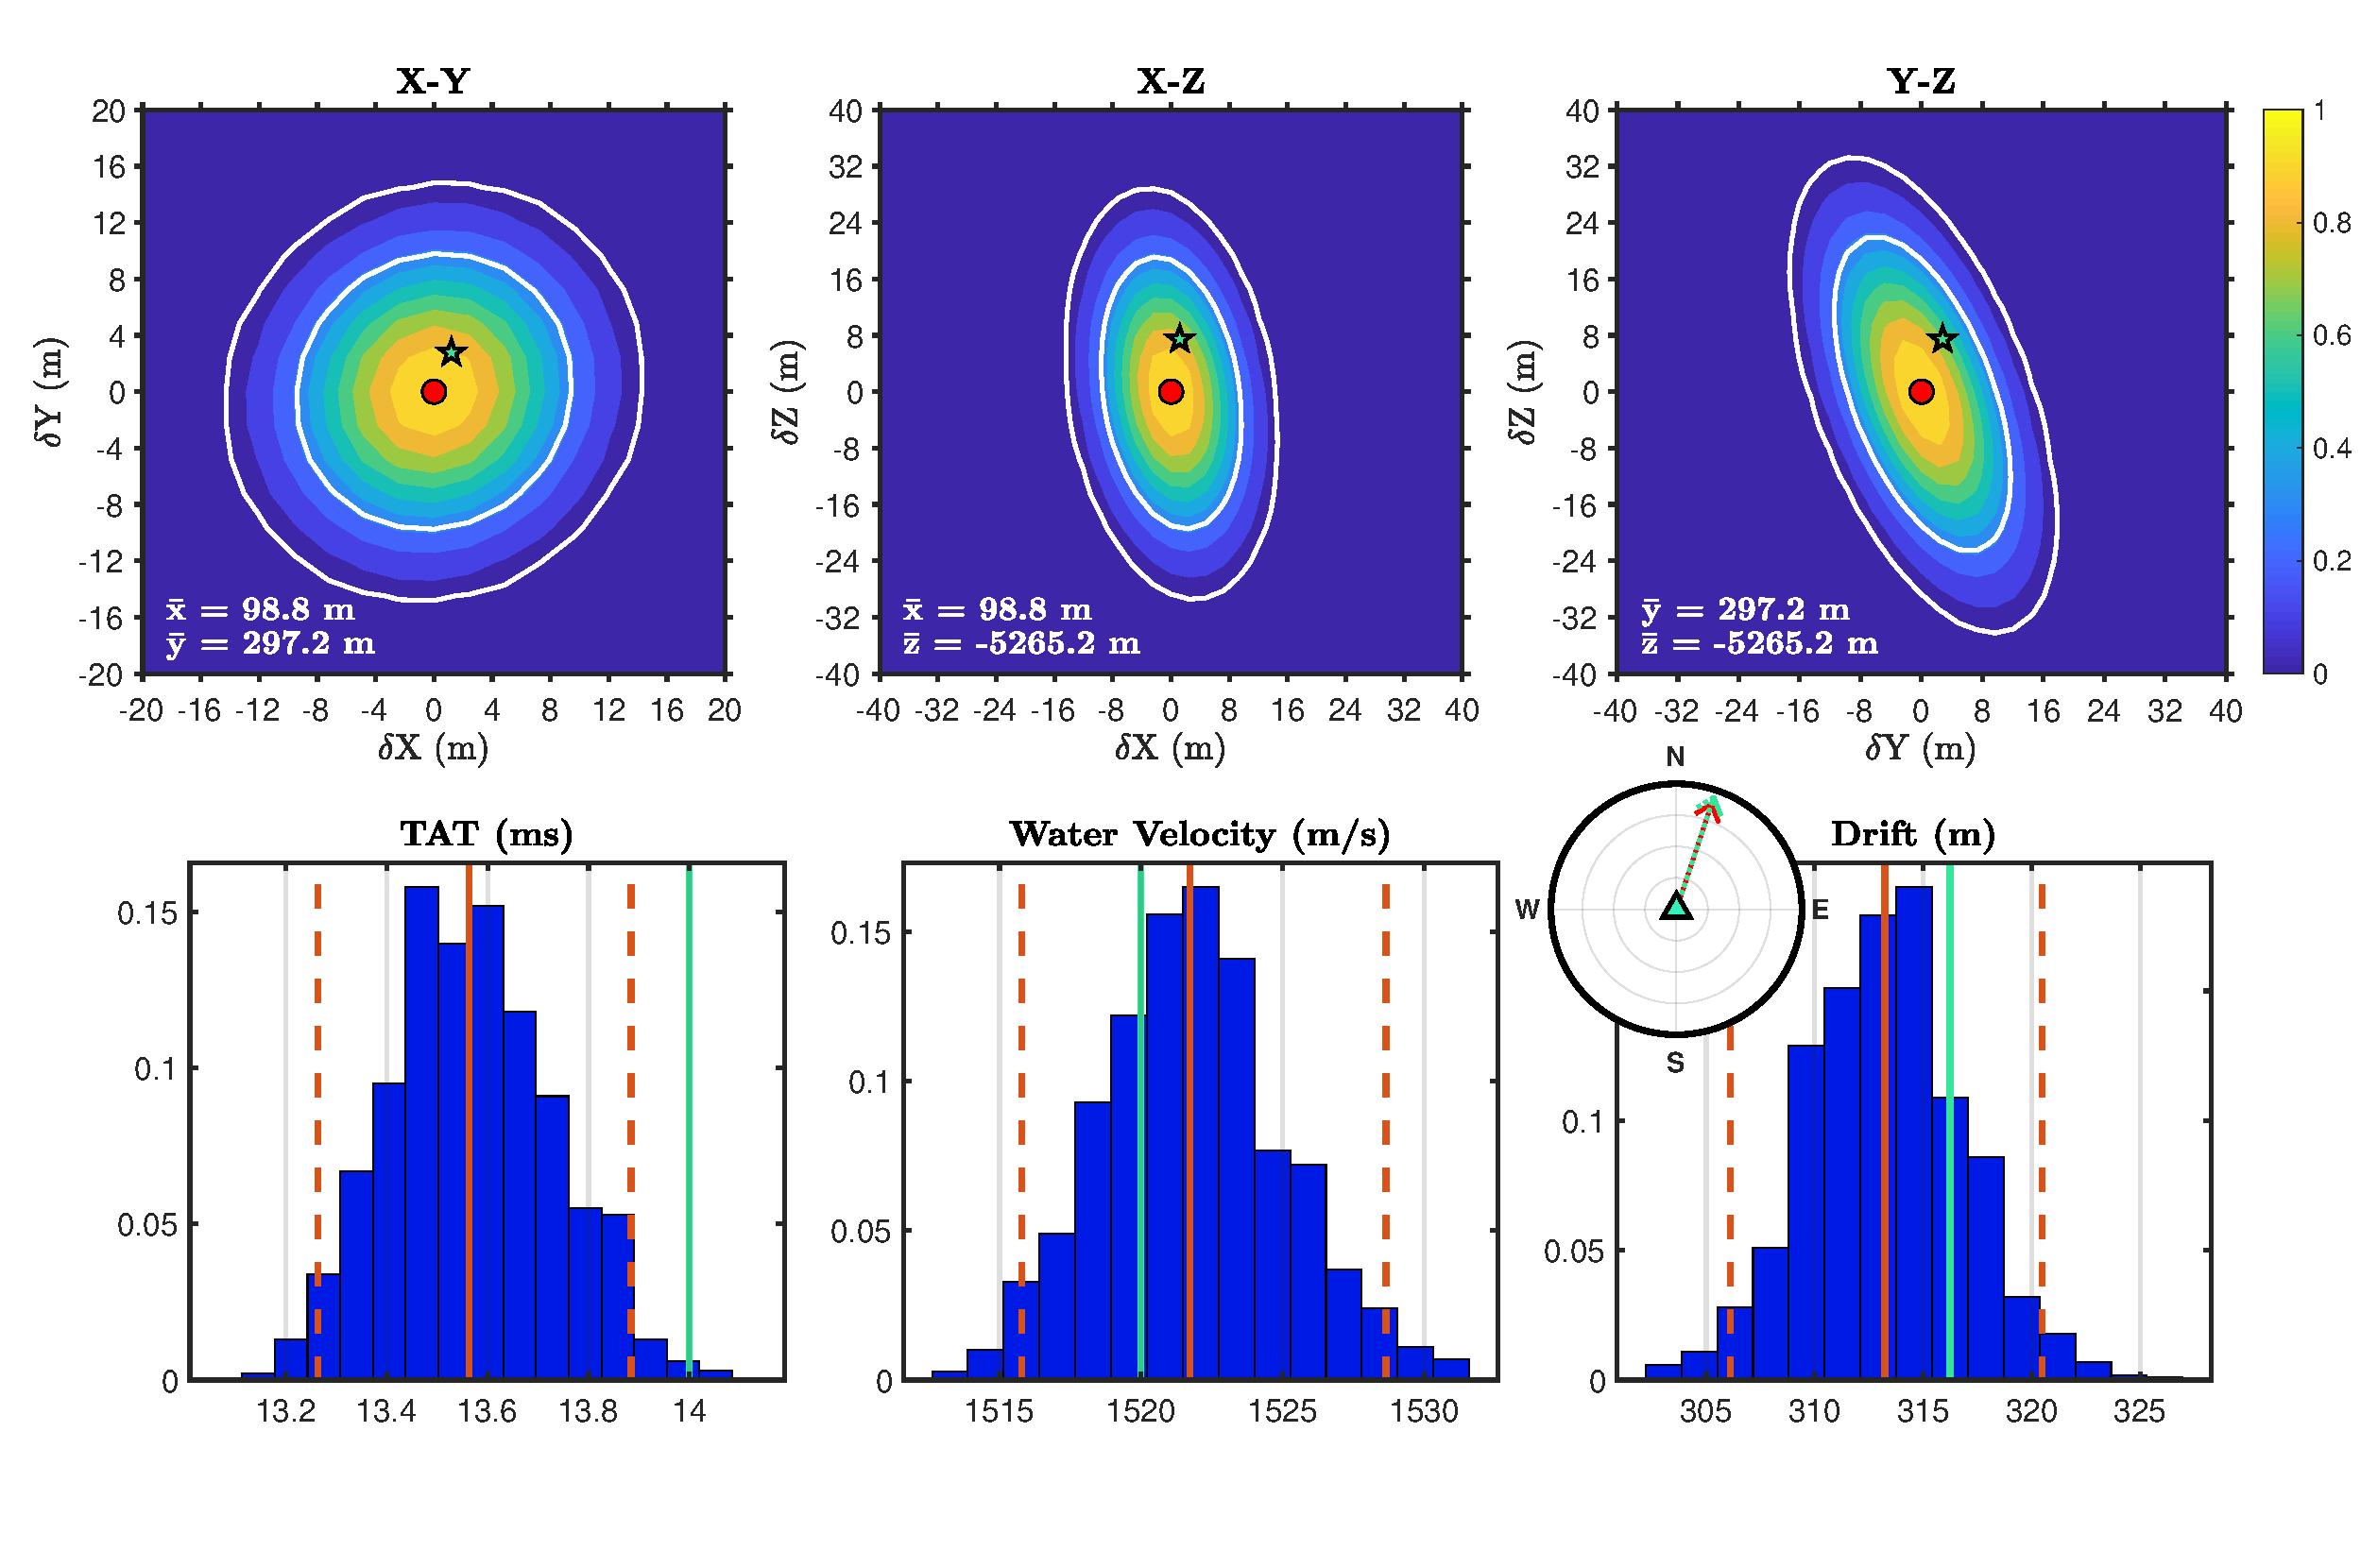
\includegraphics[trim=0cm 0cm 0cm 0cm,clip=true,width=\columnwidth]{Figure01.pdf}
\caption{Test of location algorithm using synthetic data. A comparison of the true input values (green star and lines) with the inverted model parameters (red circle and red solid lines) demonstrates that the location, depth, and water velocity are extremely well recovered, and the estimated uncertainties on these parameters are consonant with the actual misfit. Top three plots show slices through the F-test surface, contoured by probability. Bottom three plots show histograms from a bootstrap analysis with 95th percentile values indicated by dashed red lines. Inset shows the direction of true (green dashed) and estimated (red) drift with respect to the starting location. }
\label{fig:one_sta_synth}
\end{figure}

%% Example real station - survey pattern + residuals
\begin{figure}[h]
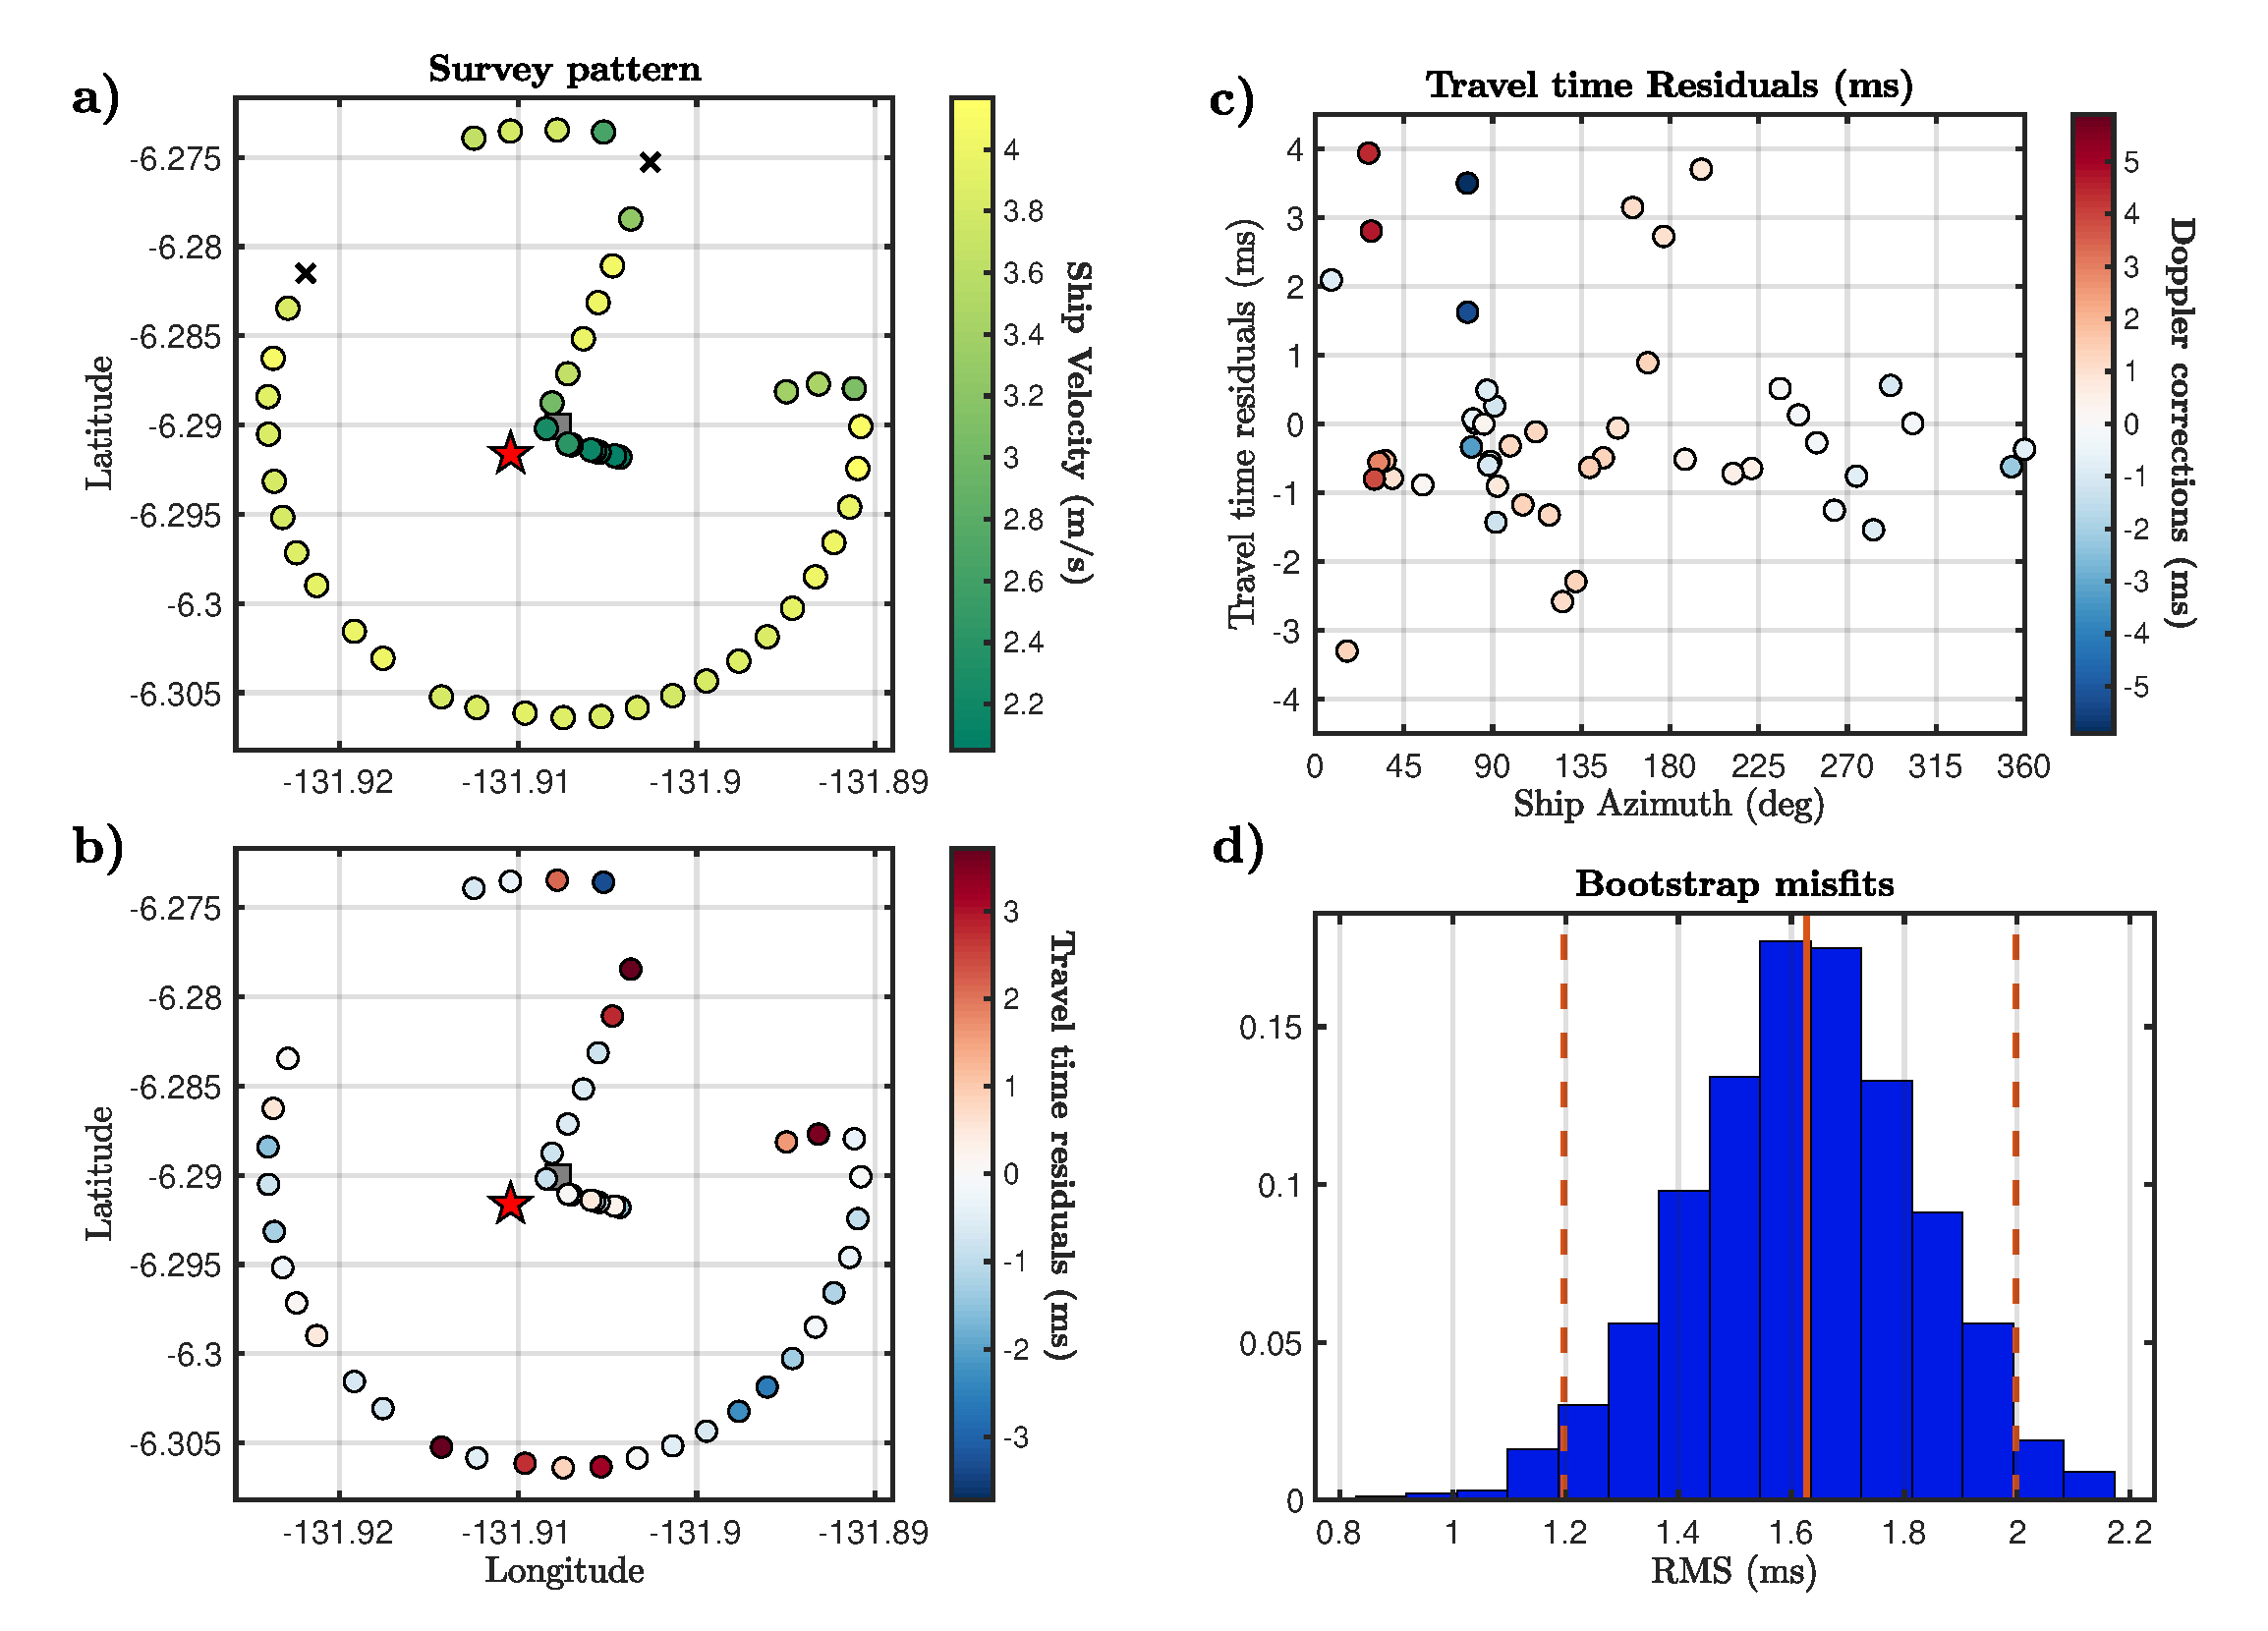
\includegraphics[trim=0cm 0cm 0cm 0cm,clip=true,width=\columnwidth]{Figure02.pdf}
\caption{Example inversion at station EC03 in the 2018 Young Pacific ORCA deployment. a) Map view of acoustic survey; colored circles are successful acoustic range measurements, black crosses are bad measurements rejected by automatic quality control, grey square is drop location, red star is final location. b) Map view of data residuals based on travel times computed using bootstrap mean station location. c) Data residuals plotted as a function of azimuth, colored by the computed doppler correction (not used in this inversion). d) Histogram of data RMS from the bootstrap; the RMS of the final model is shown as a red star.}
\label{fig:one_sta_real_survey}
\end{figure}

%% Example real station - bootstrap histogram
\begin{figure}[h]
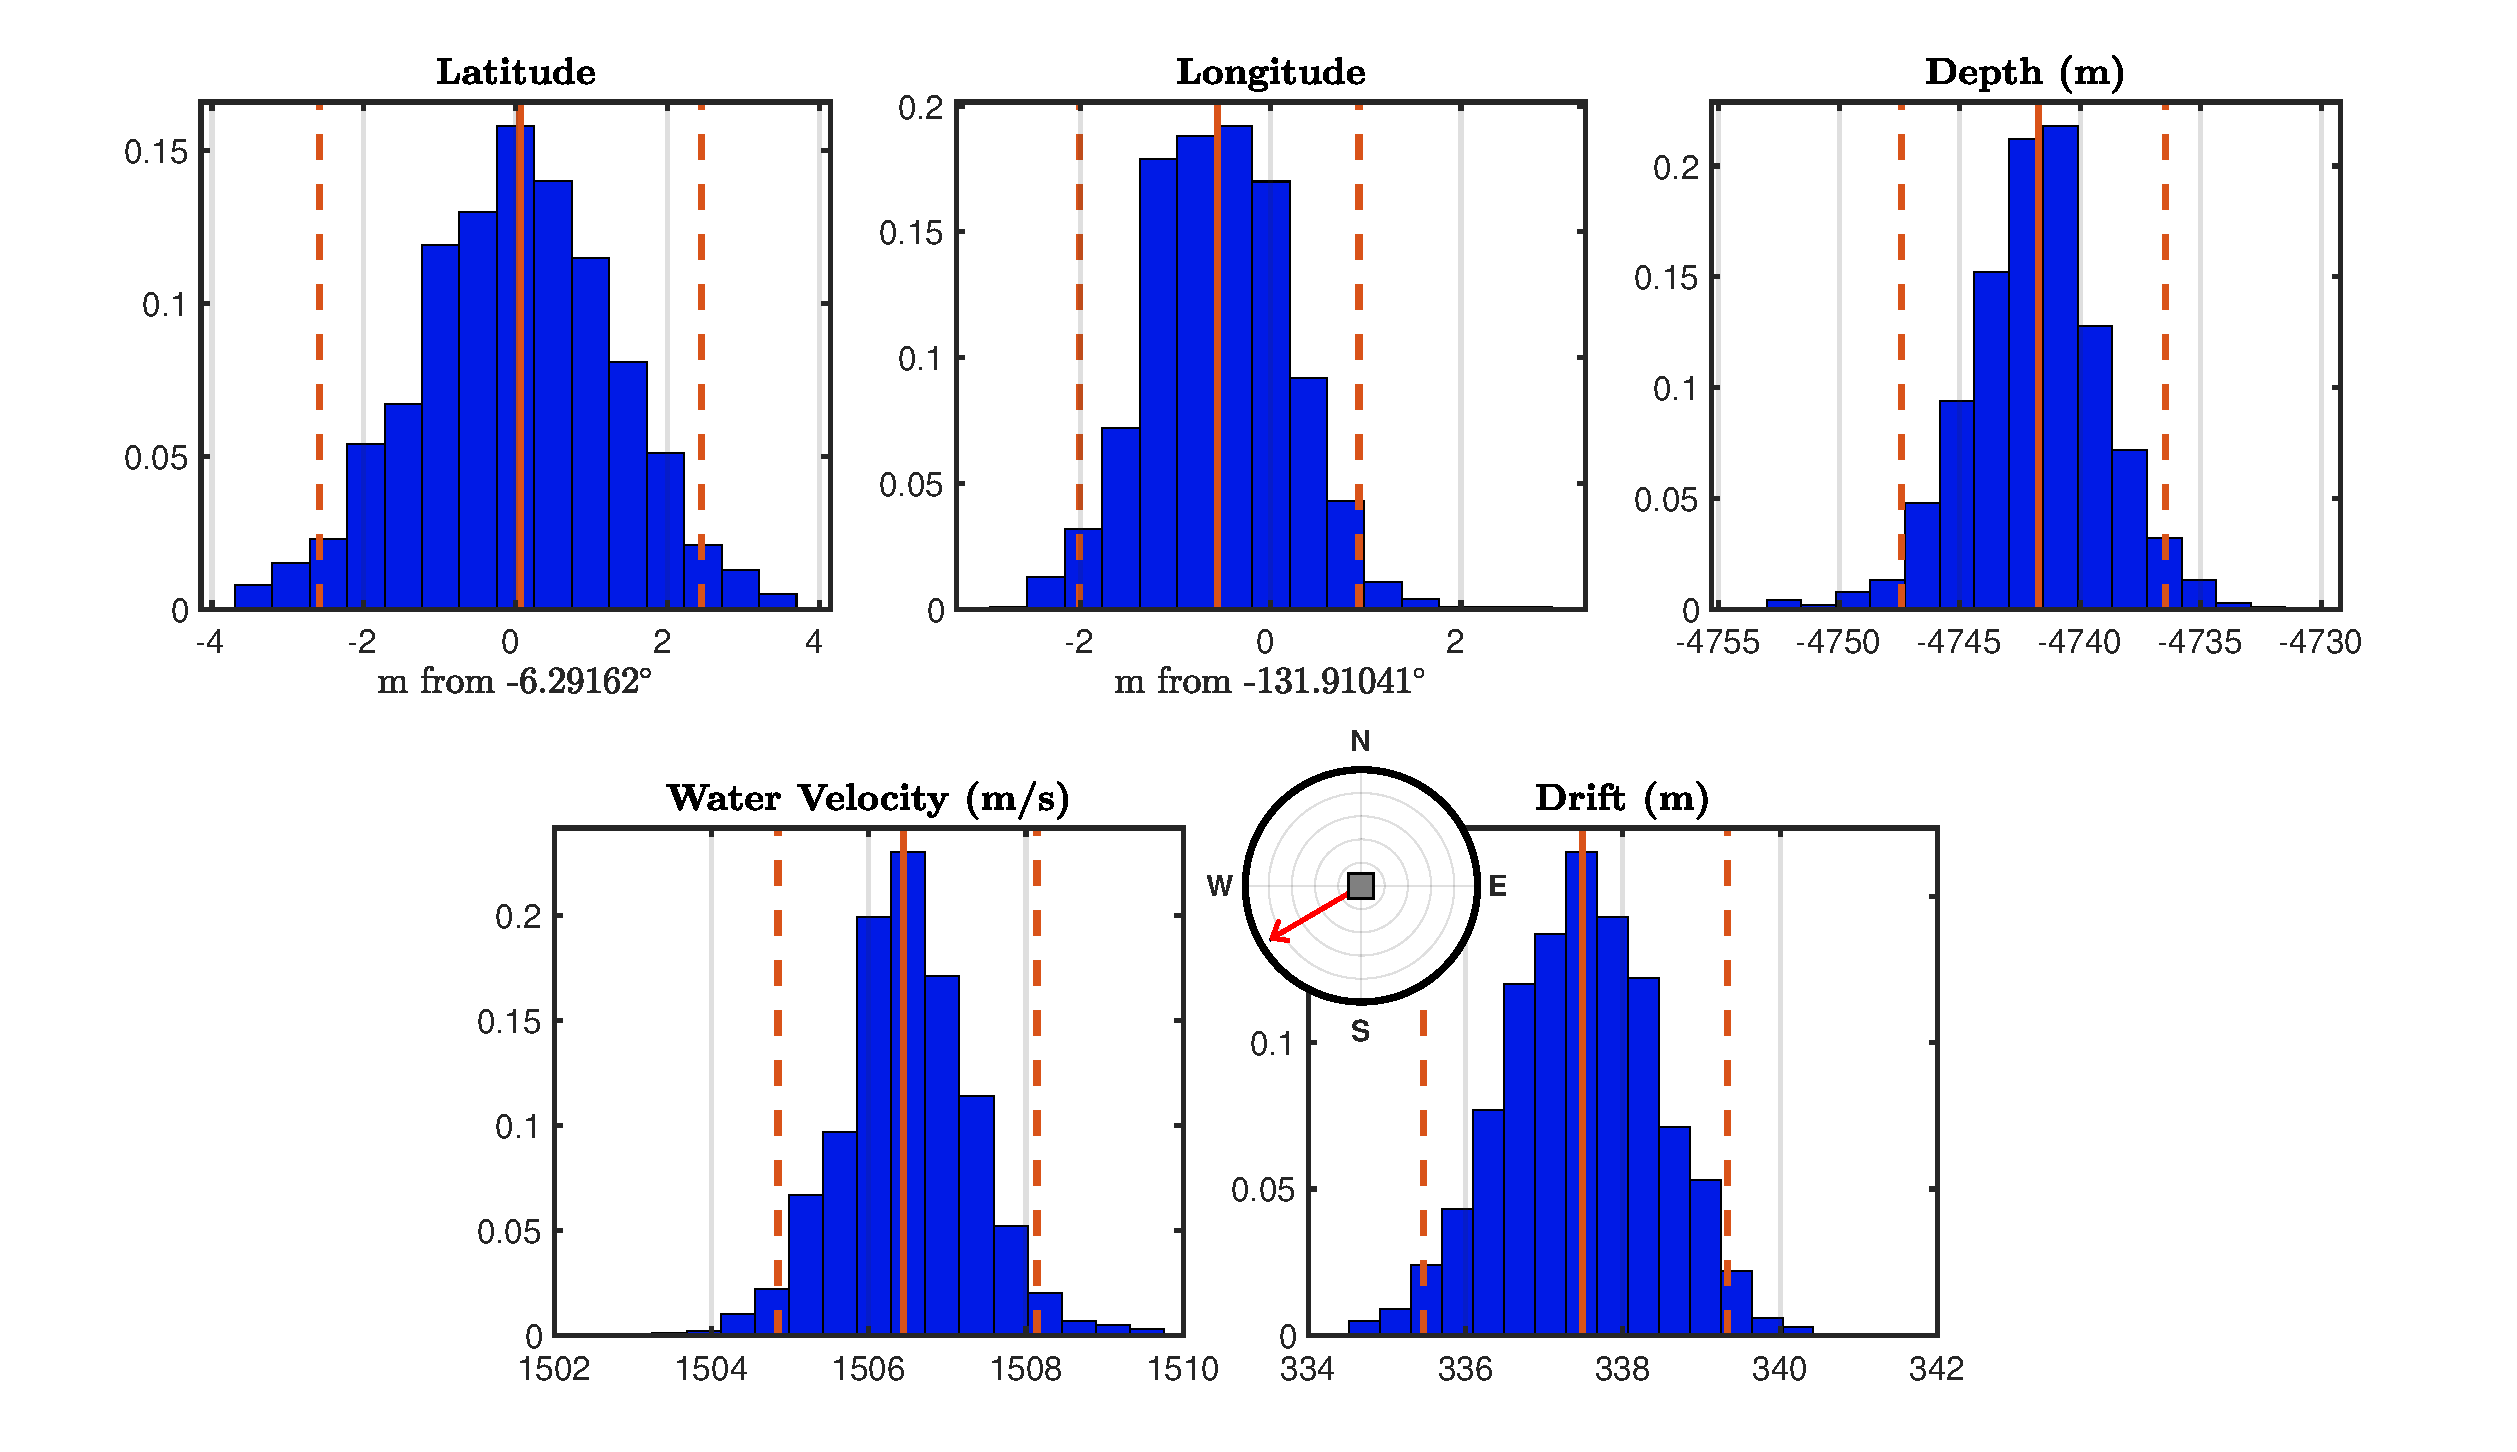
\includegraphics[trim=0cm 0cm 0cm 0cm,clip=true,width=\columnwidth]{Figure03.pdf}
\caption{Histograms of model parameters from the bootstrap inversion of station EC03 in the 2018 Young Pacific ORCA deployment. Red solid line shows mean value, while dashed lines indicate 95th percentiles. Latitude and longitude are plotted in meters from the mean point, for ease of interpretation. The inset plot shows the mean drift azimuth from the drop location (grey square).}
\label{fig:one_sta_real_histograms}
\end{figure}

%% Example real station - F-tests
\begin{figure}[h]
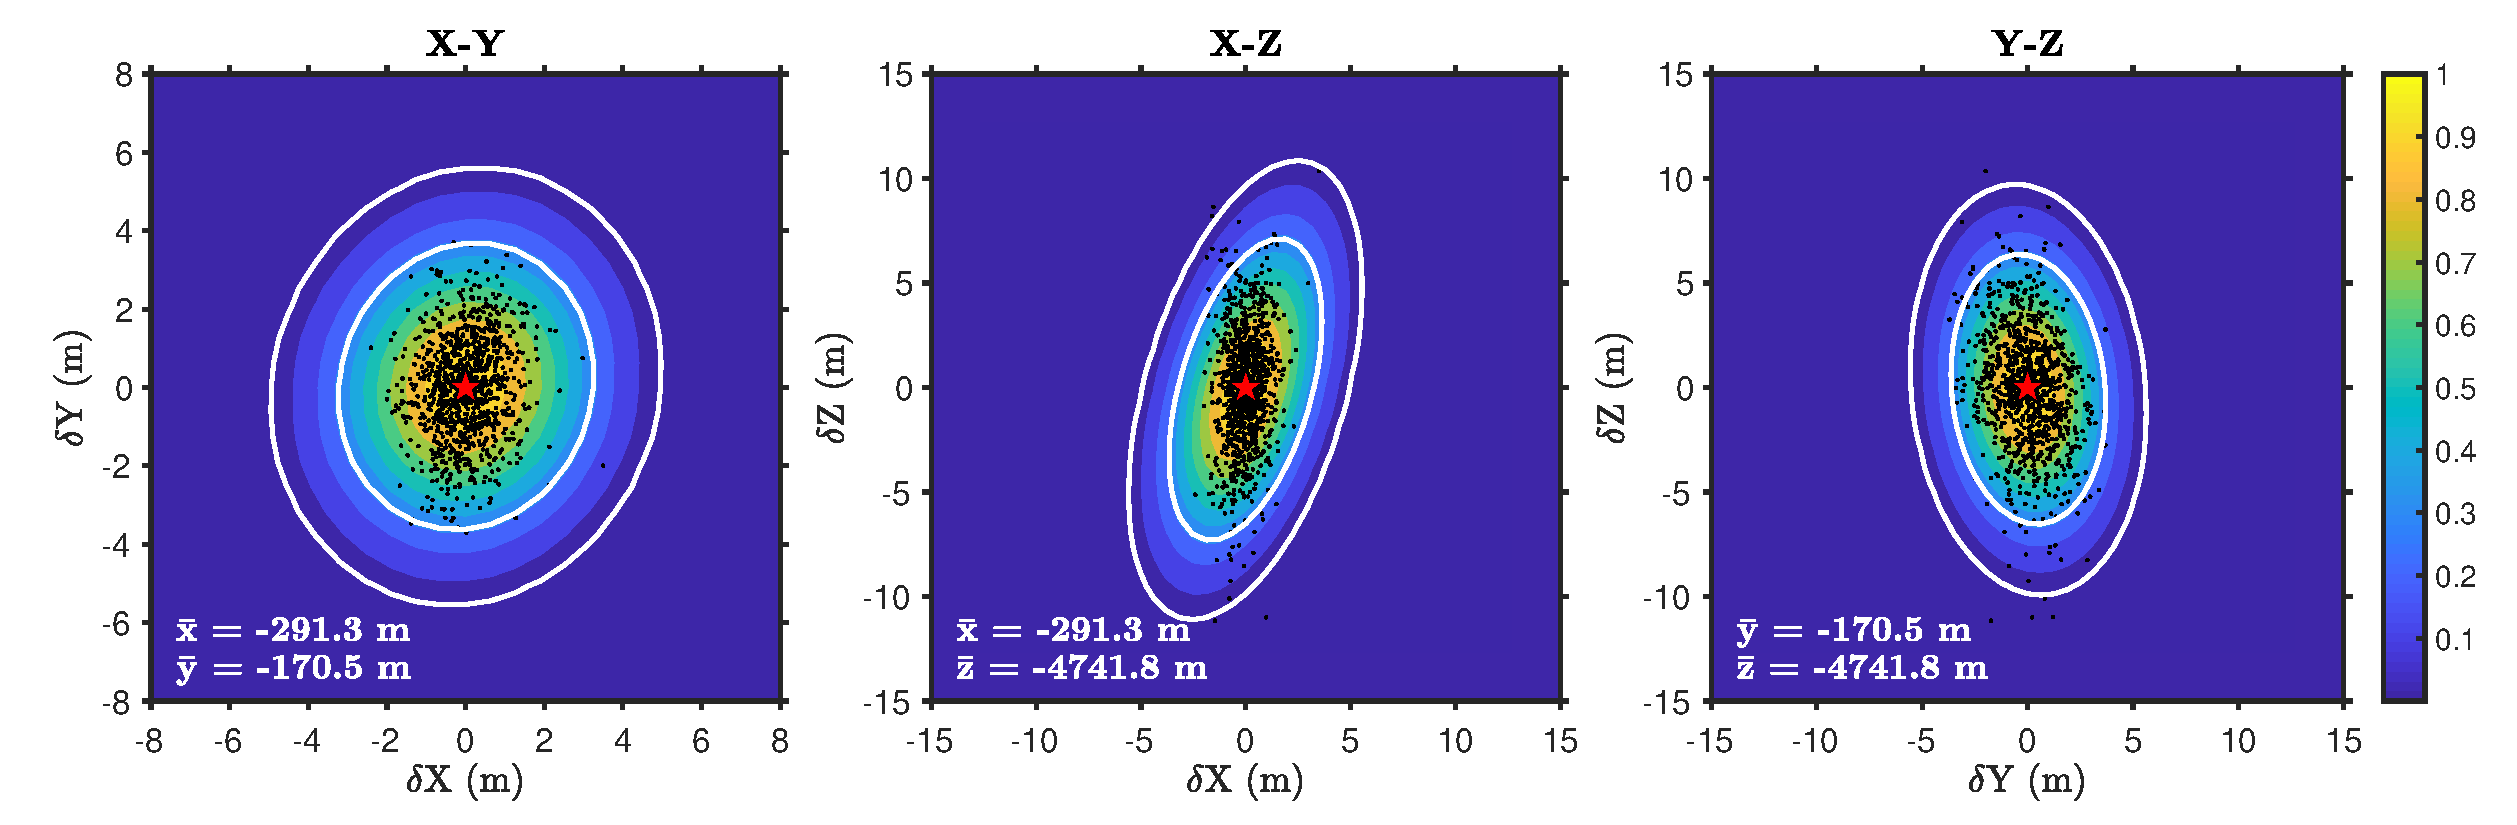
\includegraphics[trim=0cm 0cm 0cm 0cm,clip=true,width=\columnwidth]{Figure04.pdf}
\caption{ Three orthogonal slices through the F-test probability volume for station EC03 in the 2018 Young Pacific ORCA deployment, contoured by probability of true station location relative to the best fitting inverted location ($\bar{x},\bar{y},\bar{z}$), indicated by the red star. White contours show 68\% and 95\% contours. Black dots show individual locations from the bootstrap analysis (Figure \ref{fig:one_sta_real_histograms}). }
\label{fig:one_sta_real_ftests}
\end{figure}


%%% All stations meso eddy
%\begin{figure}[h]
%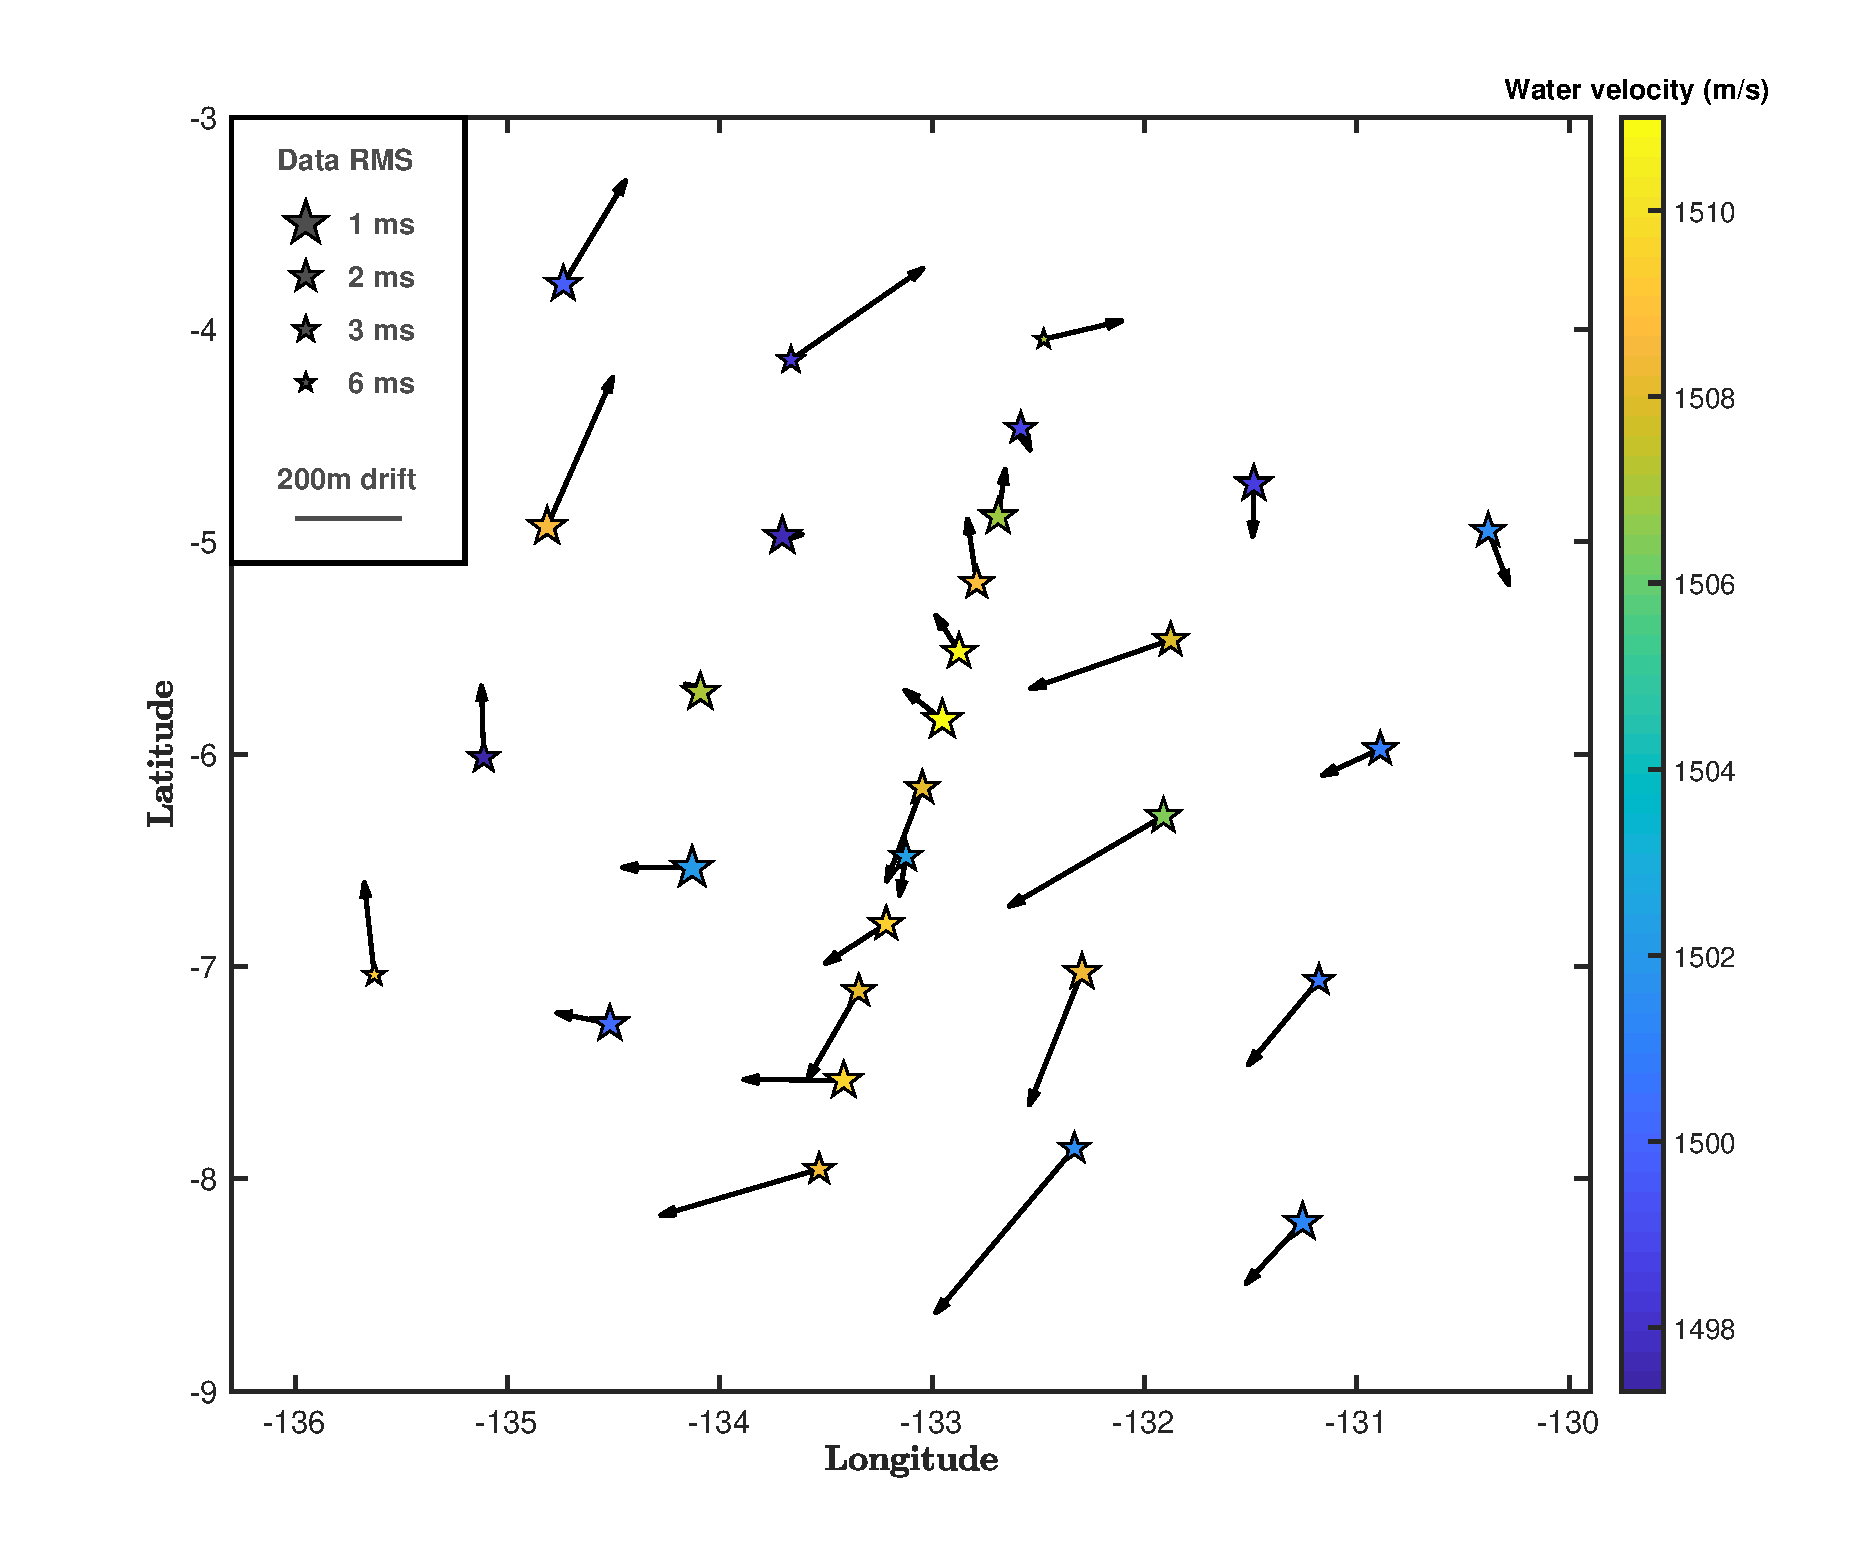
\includegraphics[trim=0cm 0cm 0cm 0cm,clip=true,width=\columnwidth]{Figure08.pdf}
%\caption{Pacific ORCA deployment, showing drift directions and magnitudes of each OBS instrument relative to their drop points, as well as the water velocity each location. Note that drift arrows are not to geographic scale. The systematic pattern of drift within the water column seems to be related to a meso-scale ocean eddy moving through this region during the deployment. Station symbol sizes are inversely scaled to acoustic travel time data misfit (see inset).}
%\label{fig:meso_eddy}
%\end{figure}

%% Comparison to previous tools
\begin{figure}[h]
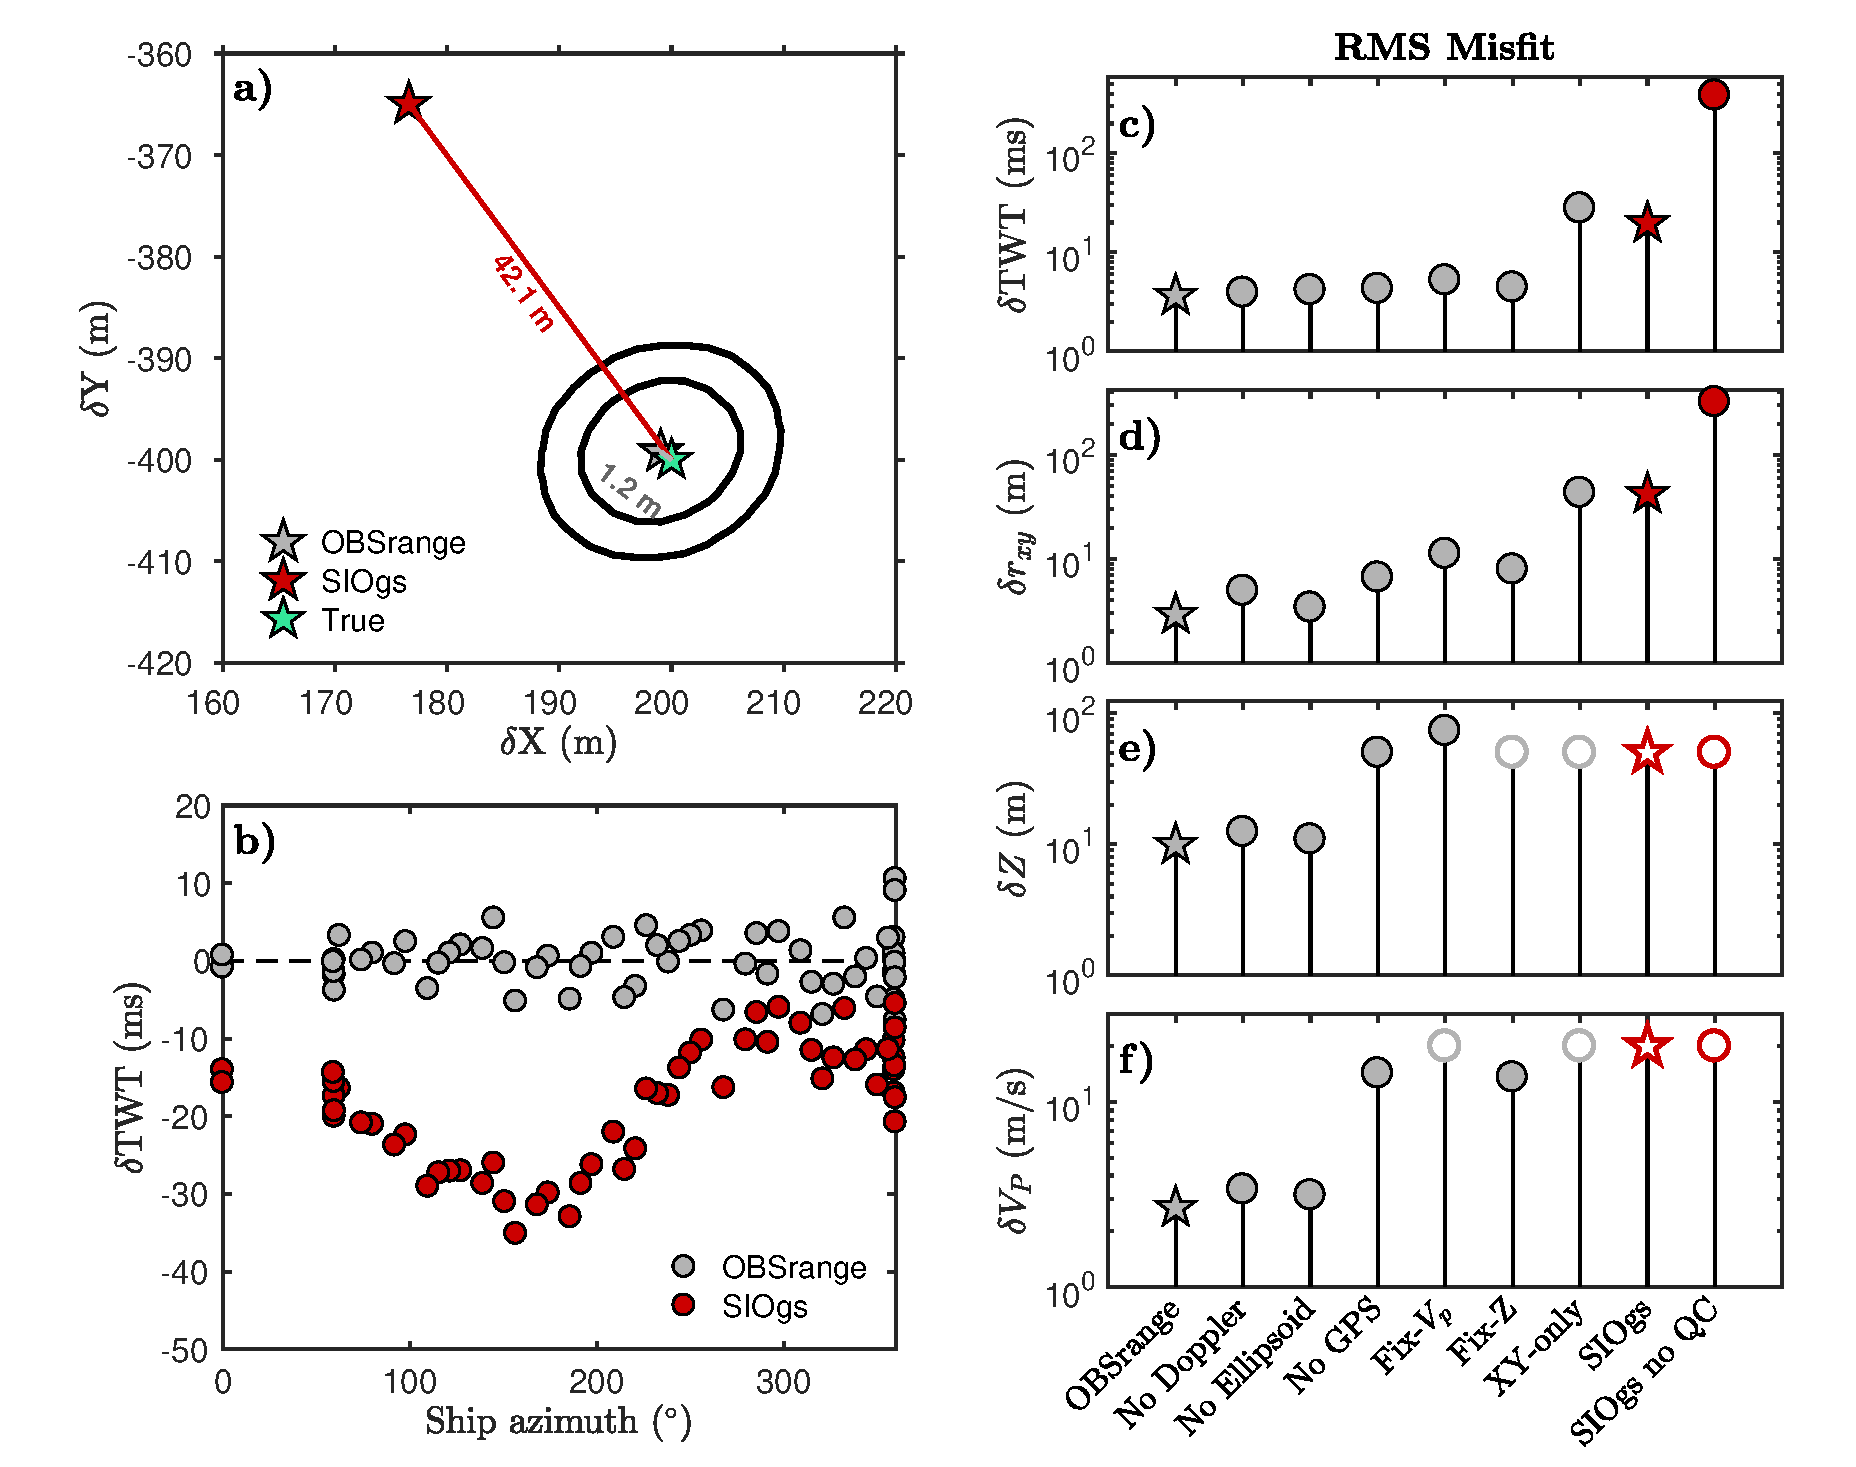
\includegraphics[trim=0cm 0cm 0cm 0cm,clip=true,width=\columnwidth]{Figure05.pdf}
\caption{ Synthetic test of OBSrange performance (gray symbols) compared with the SIO tool (red symbols) for a \textit{PACMAN} survey of radius 1 Nm. a) Map view comparing the OBSrange and SIO inverted instrument locations with the true location in green. Black contours show the 68\% and 95\% confidence from the F-test. b) Two-way time (TWT) residuals for both methods as a function of ship azimuth from the true station location. c) TWT and d--g) model parameter RMS misfits for 9 inversions, where the mislocation in $x$--$y$ is given by $\delta r_{xy} = \sqrt{\delta x_{O}^2 + \delta y_{O}^2} $. Closed symbols represent parameters that are solved for in each inversion, while open symbols denote values that remain fixed during the inversion.}
\label{fig:compare_tool}
\end{figure}

%% Exploring survey geometries
\begin{figure}[h]
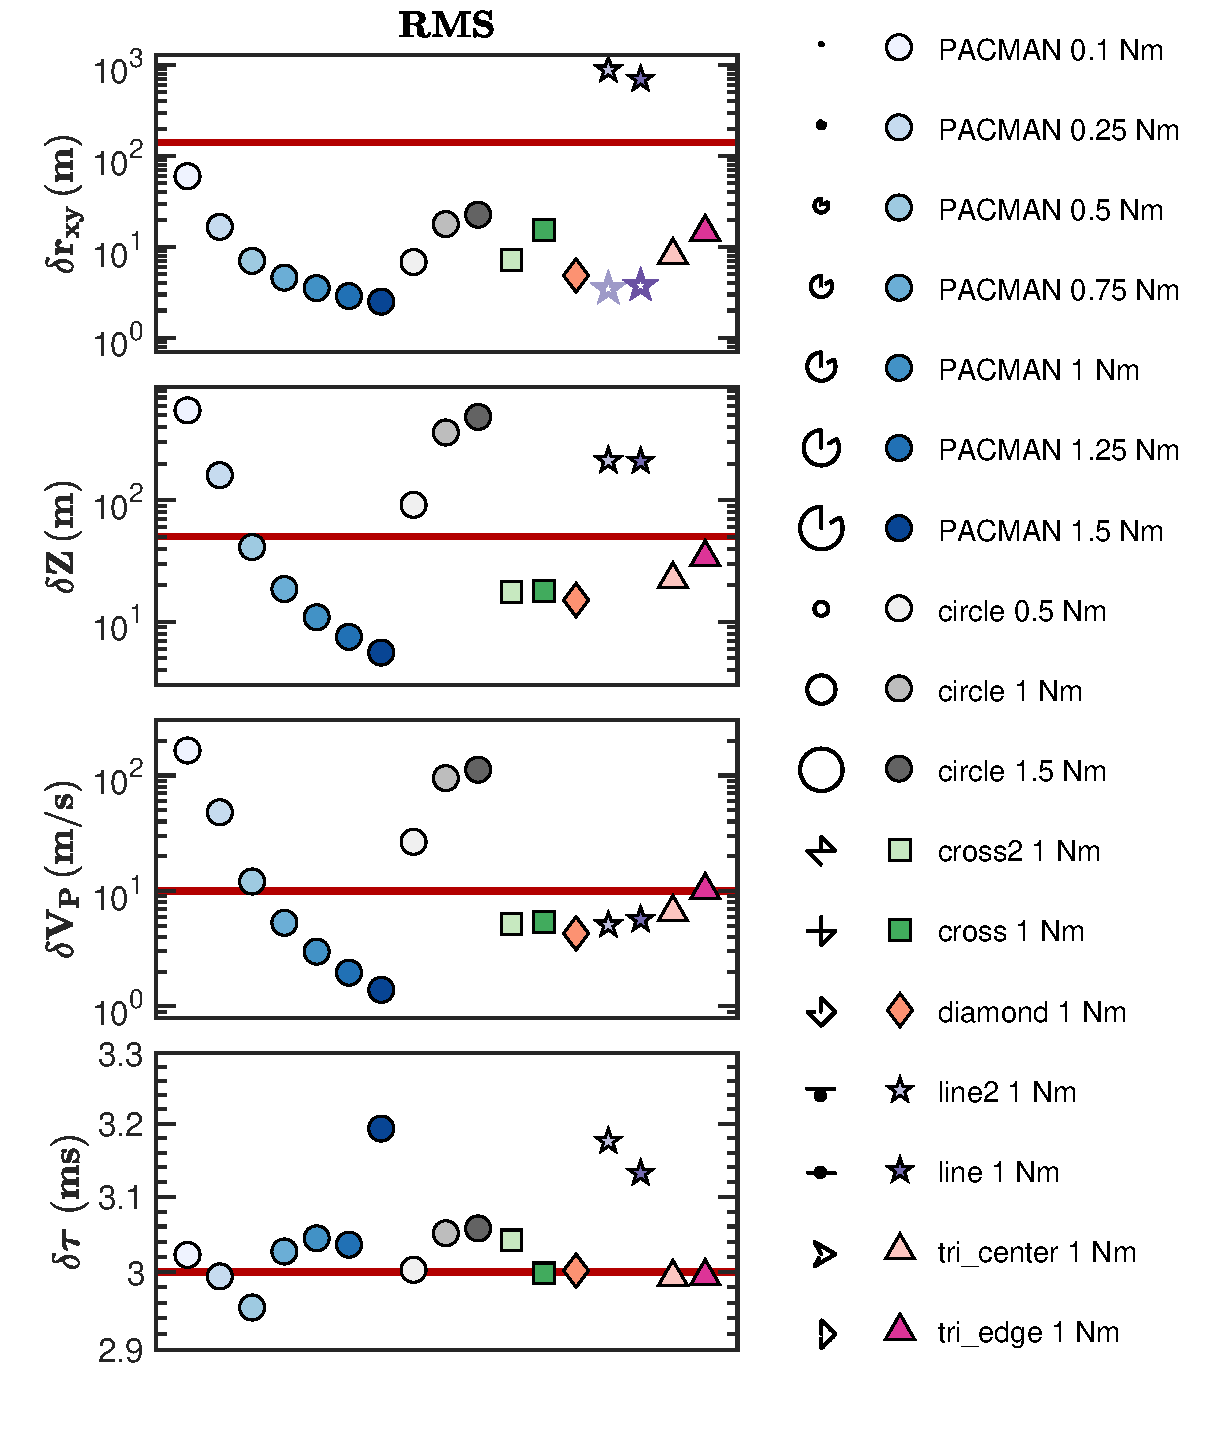
\includegraphics[trim=0cm 0cm 0cm 0cm,clip=true,width=\columnwidth]{Figure06.pdf}
\caption{ Model parameter RMS misfits for 6 synthetic survey geometries of varying radii: \textit{PACMAN}, circle, cross, diamond, line, and triangle. Each survey geometry is shown to the left of its respective legend entry. Panels show the RMS misfit for each model parameter and survey type for 10,000 synthetic survey realizations, where the mislocation in $x$--$y$ is given by $\delta r_{xy} = \sqrt{\delta x_{O}^2 + \delta y_{O}^2} $. We find that model parameters are most accurately recovered using the \textit{PACMAN} survey pattern with radius $\geq$1 Nm, and the line surveys perform worst. }
\label{fig:survey_geom_explore}
\end{figure}




\end{document}  